%=======================================================================
%  CS-3810 Design Practices in Computer Science -- Assignment 3
%  Project 3: Interactive Data Structure and Algorithms Visualizer
%  Team PY -- Papaa Dennis Morindat, Yididiya Megenta
%
%  Testing, UX and development-plan document. Sections 3-9 answer the
%  Assignment 3 brief directly. Design decisions made by the team are marked
%  [A]; requirements stated or directly implied by the project description
%  are marked [R]. The implementation is submitted separately through the
%  GitHub Classroom repository; this is the design and analysis document.
%
%  Compile with:  tectonic -X compile A3_PY.tex
%  Submission:    rename the compiled PDF to  A3_PY.pdf
%=======================================================================
\documentclass[11pt,a4paper]{article}

\usepackage[T1]{fontenc}
\usepackage{lmodern}
\usepackage[margin=2.05cm,top=2.4cm,bottom=2.4cm,headheight=14pt]{geometry}
\usepackage{amsmath,amssymb}
\usepackage{booktabs}
\usepackage{longtable}
\usepackage{array}
\usepackage{enumitem}
\usepackage{xcolor}
\usepackage{tikz}
\usetikzlibrary{arrows.meta,positioning,fit,backgrounds,calc,shapes.geometric}
\usepackage{listings}
\usepackage{caption}
\usepackage{float}          % [H]: pin floats exactly where they are written
\usepackage{fancyhdr}
\usepackage{microtype}
\usepackage{parskip}
\usepackage{titlesec}
\titlespacing*{\section}{0pt}{2.1ex plus .3ex minus .2ex}{1.0ex}
\titlespacing*{\subsection}{0pt}{1.7ex plus .2ex minus .2ex}{0.7ex}
\titlespacing*{\subsubsection}{0pt}{1.4ex plus .2ex minus .2ex}{0.5ex}
\usepackage[hidelinks]{hyperref}

\setcounter{secnumdepth}{3}
\setcounter{tocdepth}{2}
\setlength{\emergencystretch}{2em}
\setlength{\parskip}{0.35\baselineskip plus 2pt minus 1pt}
\setlength{\textfloatsep}{10pt plus 2pt minus 2pt}
\setlength{\floatsep}{10pt plus 2pt minus 2pt}
\setlength{\intextsep}{10pt plus 2pt minus 2pt}

%------------------------- colours -------------------------
\definecolor{reqc}{RGB}{0,102,51}
\definecolor{asmc}{RGB}{176,88,0}
\definecolor{primary}{RGB}{11,79,158}
\definecolor{okc}{RGB}{22,120,60}
\definecolor{warnc}{RGB}{176,88,0}
\definecolor{boxc}{RGB}{235,242,250}
\definecolor{statec}{RGB}{232,240,254}
\definecolor{rulec}{RGB}{120,120,120}
\definecolor{codec}{RGB}{245,245,247}

%------------------------- column types -------------------------
\newcolumntype{L}[1]{>{\raggedright\arraybackslash}p{#1}}
\newcolumntype{C}[1]{>{\centering\arraybackslash}p{#1}}

%------------------------- shorthands -------------------------
\newcommand{\R}{\textcolor{reqc}{\textbf{[R]}}}     % stated requirement
\newcommand{\A}{\textcolor{asmc}{\textbf{[A]}}}     % team assumption / decision
\newcommand{\ct}[1]{\texttt{#1}}
\newcommand{\bigO}[1]{\ensuremath{\mathcal{O}(#1)}}
\newcommand{\norm}[1]{\ensuremath{\lvert #1 \rvert}}
\newcommand{\done}{\textcolor{okc}{$\boxtimes$}}
\newcommand{\todo}{\textcolor{rulec}{$\square$}}

%------------------------- code listings -------------------------
\lstdefinestyle{base}{
  basicstyle=\ttfamily\footnotesize,
  columns=fullflexible,
  keepspaces=true,
  breaklines=true,
  breakatwhitespace=false,
  showstringspaces=false,
  frame=single,
  framesep=5pt,
  rulecolor=\color{rulec},
  backgroundcolor=\color{codec},
  xleftmargin=8pt,
  xrightmargin=4pt,
  aboveskip=8pt,
  belowskip=8pt
}
\lstset{style=base}
\lstset{floatplacement=H}
\lstdefinestyle{pseudo}{style=base,numbers=left,numberstyle=\tiny\color{rulec},numbersep=6pt}
\lstdefinestyle{ts}{style=base,numbers=none}
\lstdefinestyle{c}{style=base,numbers=left,numberstyle=\tiny\color{rulec},numbersep=6pt,
  language=C,keywordstyle=\color{primary}\bfseries,
  commentstyle=\color{rulec}\itshape,stringstyle=\color{asmc}}
\lstdefinestyle{sh}{style=base,numbers=none}

\captionsetup{font=small,labelfont=bf,skip=4pt}
\renewcommand{\arraystretch}{1.06}

%------------------------- tikz styles -------------------------
\tikzset{
  comp/.style={draw=rulec, rounded corners=2pt, fill=boxc, align=center,
               inner sep=5pt, font=\small, text width=3.6cm, minimum height=1.35cm},
  layer/.style={draw=rulec, rounded corners=2pt, fill=boxc, align=left,
                inner sep=6pt, font=\small, text width=14.2cm},
  auxbox/.style={draw=rulec, rounded corners=2pt, fill=statec, align=center,
                 inner sep=4pt, font=\footnotesize},
  wf/.style={draw=rulec, fill=white, align=center, inner sep=2pt, font=\scriptsize},
  wfh/.style={draw=rulec, fill=statec, align=center, inner sep=2pt,
              font=\scriptsize\bfseries},
  n/.style={circle, draw=rulec, fill=white, inner sep=1pt, minimum size=4.6mm,
            font=\scriptsize},
  nactive/.style={circle, draw=primary, very thick, fill=statec, inner sep=1pt,
                  minimum size=4.6mm, font=\scriptsize},
  e/.style={-{Stealth[length=2.2mm]}, draw=rulec, thick},
  ed/.style={-{Stealth[length=2.2mm]}, draw=rulec!70, dashed},
  ebi/.style={{Stealth[length=2.2mm]}-{Stealth[length=2.2mm]}, draw=rulec},
  lbl/.style={font=\scriptsize, inner sep=1.6pt, fill=white}
}

%------------------------- headers -------------------------
\pagestyle{fancy}
\fancyhf{}
\fancyhead[L]{\footnotesize CS-3810: Design Practices in Computer Science}
\fancyhead[R]{\footnotesize Assignment 3: Testing, UX, and Development Plan}
\fancyfoot[C]{\footnotesize\thepage}
\renewcommand{\headrulewidth}{0.3pt}

\begin{document}

%=======================================================================
\begin{center}
  {\large\bfseries Department of Computer Science}\\[2pt]
  {\small Ashoka University}\\[10pt]
  {\LARGE\bfseries CS-3810: Design Practices in Computer Science}\\[6pt]
  {\large\bfseries Assignment 3: Testing, UX, and Development Plan}\\[10pt]
  {\large\bfseries Project 3: Interactive Data Structure and Algorithms Visualizer}
\end{center}

\vspace{2pt}
\begin{center}
\renewcommand{\arraystretch}{1.25}
\begin{tabular}{@{}L{4.2cm}L{10.4cm}@{}}
\toprule
\textbf{Assignment Type} & Group Assignment \\
\textbf{Marks} & 100 \\
\textbf{Submission Format} & PDF generated from \LaTeX \\
\textbf{Submission} & Google Classroom \\
\textbf{Naming Convention} & A3\_PY.pdf \\
\bottomrule
\end{tabular}
\end{center}

%-----------------------------------------------------------------------
\noindent\textbf{Markers.} \R\ --- a requirement stated or directly implied by the project
description; \A\ --- an assumption, design decision or target made by the team. Requirement,
error and non-functional identifiers (FR, ER, NFR, UC) are those of \ct{A1\_PY.tex}; ADR
identifiers are those of \ct{A2\_PY.tex}.

\tableofcontents

%=======================================================================
\section{Project Identification}

\begin{center}
\renewcommand{\arraystretch}{1.25}
\begin{tabular}{@{}L{4.2cm}L{10.4cm}@{}}
\toprule
\textbf{Team Name} & PY. \\
\textbf{Team Members} & Papaa Dennis Morindat, Yididiya Megenta \\
\textbf{Roll Numbers} & 1020241748, 1020241852 \\
\textbf{Assigned Project} & Project 3: Interactive Data Structure and Algorithms Visualizer \\
\textbf{Repository Link} & \url{https://github.com/Ashoka-CS-3810-Design-Practices-in-CS/project-3-PY} \\
\bottomrule
\end{tabular}
\end{center}

\subsection{Assigned Project}

\noindent\textbf{Project title.} Interactive Data Structure and Algorithms Visualizer.

\medskip
\noindent\textbf{Problem statement.} \R\ A data-structures course leaves the learner with the
final answer --- a tree, a sorted array, a visit order --- but the misunderstanding lives in
the transient state: which pointer is followed, what is on the call stack or in the queue,
which vertices are discovered, and how many comparisons were spent. That state is invisible
on a whiteboard, laborious to draw, and impossible to rewind.

\medskip
\noindent\textbf{Motivation.} \R\ Three observations drive the project. (i)~The result does
not teach the method: a min-heap array after six insertions says nothing about why each
sift-up stopped. (ii)~Misconceptions are about process, not outcome: ``BFS jumps to the
nearest unvisited node'' is a claim about intermediate states. (iii)~Manual tracing does not
scale, so it teaches the wrong habit. A visualiser whose intermediate states are wrong is
therefore worse than none, which is why \S3 treats trace correctness as a first-class
requirement.

\medskip
\noindent\textbf{Intended users.} \R\ Primary: second-year undergraduates meeting the
pseudocode for the first time. Secondary: instructors and teaching assistants demonstrating
live, including worst cases. Tertiary: self-learners and interview candidates revising.

\medskip
\noindent\textbf{Main goal of the application.} \R\ An interactive, step-controlled
visualiser: the user selects a structure and an operation, supplies or loads a dataset, and
watches it execute one step at a time with the structural view, the algorithm line and the
auxiliary state (array, stack, queue, heap, visited set, call stack) advancing in lockstep,
with a plain-English explanation and the time and space complexity.

%=======================================================================
\section{Purpose of the Assignment}

\R\ This is the third design-stage deliverable. It translates the Assignment~2 design into an
executable plan for correctness and testing (\S3), complexity and performance (\S4), user
interaction (\S5), risk (\S6), development and integration (\S7) and delivery (\S8), and it
closes with the design-review answers (\S9) and the submission checklist (\S10).

The plan leans on one property of that design: an operation is a pure function that emits a
serialisable, deterministic \ct{Step[]}. The core is therefore tested in Node with no browser,
a committed JSON fixture is a regression oracle, and a UI test is a comparison of two renders
rather than a simulation of an animation. \A\ Where a target cannot yet be met by the current
vertical slice, the section says so and names the phase in \S7 that owns it.

%=======================================================================
\section{Correctness and Testing Plan}

The brief asks how correctness will be established, how the major algorithms and components
will be tested, and which boundary, invalid-input, algorithm-specific, interaction and
performance cases matter. This section answers those questions in the order the brief gives
them, and closes with representative test cases and the coverage and CI gates.

\subsection{Testing strategy and levels}

\A\ We use the test pyramid of Figure~\ref{fig:pyramid}: a large base of fast, DOM-free unit
and property tests over pure functions, a middle of integration tests over the request
pipeline and the storage layer, and a thin top of UI and end-to-end tests. The distribution
is not stylistic. The architecture of Assignment~2 \S5 puts the pedagogical content in the
algorithm and model layers, so that is where the risk is and where the tests should be; and
because those layers are pure functions of plain data, their tests are deterministic, fast
and runnable in CI without a browser. Screenshot tests are deliberately absent
(Assignment~2 \S6): the visual output is expected to change frequently, whereas a golden
\emph{trace} is a stable, readable regression diff.

\begin{figure}[htbp]
\centering
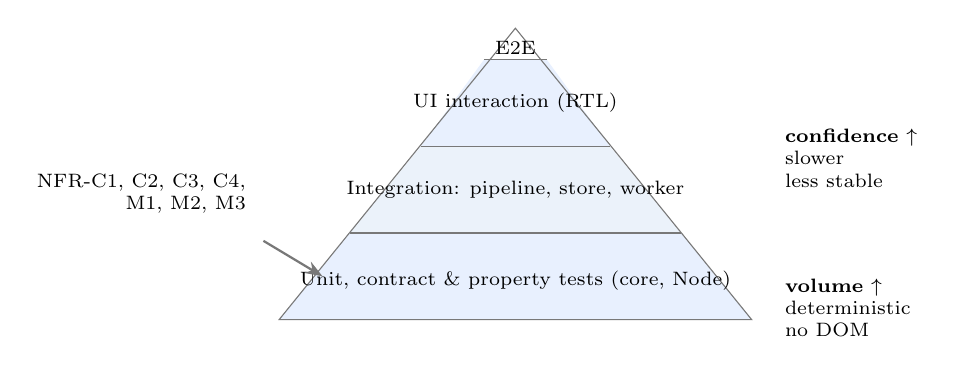
\begin{tikzpicture}[font=\scriptsize]
  % pyramid bands
  \fill[statec] (0,0) -- (6,0) -- (5.1,1.1) -- (0.9,1.1) -- cycle;
  \fill[boxc]   (0.9,1.1) -- (5.1,1.1) -- (4.2,2.2) -- (1.8,2.2) -- cycle;
  \fill[statec] (1.8,2.2) -- (4.2,2.2) -- (3.4,3.3) -- (2.6,3.3) -- cycle;
  \draw[rulec] (0,0) -- (6,0) -- (3,3.7) -- cycle;
  \draw[rulec] (0.9,1.1) -- (5.1,1.1);
  \draw[rulec] (1.8,2.2) -- (4.2,2.2);
  \draw[rulec] (2.6,3.3) -- (3.4,3.3);
  \node at (3,0.5) {Unit, contract \& property tests (core, Node)};
  \node at (3,1.65) {Integration: pipeline, store, worker};
  \node at (3,2.75) {UI interaction (RTL)};
  \node[align=center] at (3,3.45) {E2E};
  % side annotations
  \node[align=left, anchor=west] at (6.3,0.15) {\textbf{volume} $\uparrow$\\ deterministic \\ no DOM};
  \node[align=left, anchor=west] at (6.3,2.05) {\textbf{confidence} $\uparrow$\\ slower \\ less stable};
  \node[align=right, anchor=east] at (-0.3,1.6) {NFR-C1, C2, C3, C4,\\ M1, M2, M3};
  \draw[e] (-0.2,1.0) -- (0.55,0.55);
\end{tikzpicture}
\caption{The test pyramid. The wide base is the DOM-free core, which is where the graded
pedagogy lives; the narrow top is one end-to-end walkthrough. The arrow marks where the
correctness non-functional requirements (NFR-C1--C4) are enforced.}
\label{fig:pyramid}
\end{figure}

\noindent Table~\ref{tab:levels} is the level-by-level plan. ``Evidence'' distinguishes what
already exists in the repository from what a later phase of Section~7 will add; a grader can
therefore check the claim rather than take it on trust.

{\footnotesize
\setlength{\tabcolsep}{4pt}
\begin{longtable}{@{}L{0.9cm}L{3.2cm}L{3.5cm}L{3.9cm}L{3.2cm}@{}}
\caption{The nine test levels. Levels L0, L1 (list) and L2 (one operation) and L4 already
exist in the repository and run in CI; the rest are scheduled by Section~7.}\label{tab:levels}\\
\toprule
\textbf{Level} & \textbf{What it tests} & \textbf{Tool / scope} & \textbf{What a pass proves} &
\textbf{Status and evidence} \\
\midrule
\endfirsthead
\toprule
\textbf{Level} & \textbf{What it tests} & \textbf{Tool / scope} & \textbf{What a pass proves} &
\textbf{Status and evidence} \\
\midrule
\endhead
\bottomrule
\endlastfoot
L0 & \ct{Step} contract: exact key set, closed \ct{EdgeKind}/\ct{AuxKind} unions, JSON
round-trip, \ct{@}-field separation & Vitest, Node; \ct{core/trace/} &
Generator and renderer cannot drift; the contract cannot change silently &
\done\ \ct{step.test.ts}, 6 tests \\
L1 & Model invariants: list linkage and acyclicity, stack LIFO, heap property, BST ordering,
graph has no self-loop & Vitest, Node; \ct{core/model/} &
Each structure is internally consistent before any algorithm touches it &
\done\ for the list (7 tests); planned per structure \\
L2 & Unit emission: step sequence, one step per meaningful pseudocode line, delta contents,
narration, \ct{GenerateSummary} & Vitest, Node; \ct{core/ops/} &
The trace describes the algorithm that was specified in Assignment~2 \S3 &
\done\ for \ct{insertAtHead} (7 tests); planned per operation \\
L3 & Differential and property tests against independent oracles (\S3.2) & Vitest +
\ct{fast-check}; core & Generated trace results agree with a reference implementation for
randomised inputs, not just the examples we thought of &
Partial: determinism and non-mutation tested; oracle harness planned \\
L4 & Trace storage: \ct{reconstruct(i)} equals replay-from-zero for every $i$; checkpoint
correctness; non-mutation of checkpoints & Vitest + \ct{fast-check}; \ct{core/trace/} &
Step-back, scrub and exact replay are correct by construction, not by luck &
\done\ \ct{store.test.ts}, 5 tests \\
L5 & Integration, request pipeline: parse $\to$ validate $\to$ build $\to$ execute $\to$
\ct{controller.load}; no raw text reaches the engine & Vitest, Node; \ct{app/} &
FR6 and ADR-7 hold end to end: the engine can assume well-typed input &
Planned (Phase~3); the pipeline exists for the slice \\
L6 & Worker boundary: \ct{GenerateRequest} / \ct{GenerateResponse} structured-clone; error
propagation; worker terminated on reset & Vitest; \ct{app/worker*} &
Large inputs do not block the main thread and cannot leak a background computation &
Planned (Phase~3) \\
L7 & UI interaction: panes synchronised to one index; controls and keyboard; disabled states;
ARIA live region; error-boundary containment; reduced motion & React Testing Library,
\ct{jsdom}; \ct{ui/} & FR8--FR11 and NFR-U2 are real interactions, not markup that merely
looks right & Planned (Phase~4) \\
L8 & End-to-end: one full user journey in a real browser & Playwright; \ct{tests/e2e/} &
The assembled product works for the UC1 $\to$ UC2 flow (NFR-U1) &
Planned (Phase~5); \ct{@playwright/test} is installed \\
L9 & Performance: generation latency, frame time, payload, memory, reconstruction work &
Vitest bench + a budget script + Lighthouse; \ct{perf/} &
The numeric targets of Section~4 are measured and enforced, not asserted &
Planned (Phase~5) \\
\end{longtable}
}

\subsection{Test oracles: how ``correct'' is decided}

A test is only as good as its oracle: it is easy to test that an animation renders, and hard to
test that it is \emph{true}. We use five oracles, and every algorithmic test names the one it
uses.

\begin{enumerate}[leftmargin=1.6em,topsep=2pt,itemsep=2pt]
  \item \textbf{Invariant oracle.} \R\ A pure predicate per structure must hold after
        \emph{every} step, not only at the end (NFR-C4): the heap property at every
        parent/child pair, the BST ordering at every node, list acyclicity and
        single-predecessor linkage, LIFO for the stack, FIFO for the queue, no self-loop or
        duplicate edge, and acyclic parent links in a depth-first forest. The same predicate is
        reused by the generator test, the property tests and the golden-trace test.
  \item \textbf{Independent reference implementation.} \R\ Each operation is re-implemented in
        the simplest obviously-correct way --- an array for a list, a sorted array for
        extract-min, a textbook recursion for a traversal --- with no instrumentation and no
        shared code. The structure reconstructed from the trace must equal the reference
        result (NFR-C1).
  \item \textbf{The C reference functions of Assignment~2 \S3.} \A\ The textbook C functions are
        compiled against a fixed fixture and their visit sequence and final structure compared
        with the trace, so instrumentation is shown to change only what is \emph{recorded},
        never what is \emph{computed}.
  \item \textbf{Golden traces.} \R\ Because the trace is deterministic (ADR-8, NFR-C2), a
        committed JSON fixture is an exact regression oracle: a behaviour change is a readable
        diff a reviewer approves, and a pure refactor produces no diff. The repository already
        holds \ct{src/data/golden/list-insertAtHead.json}; every operation will hold one.
  \item \textbf{Metamorphic relations.} \A\ Cheap-to-state properties turn two algorithms into
        each other's oracle: inorder of a BST equals the sorted key set; level-order equals BFS
        on the same tree; iterative and recursive DFS agree; extracting a min-heap yields
        ascending order; reversing a list twice is the identity; search finds exactly the keys
        inserted.
\end{enumerate}

\begin{lstlisting}[style=ts,caption={The invariant oracle in the shape every structure
follows: a pure predicate over the model, asserted in the generator test (here, the min-heap
property) and reused by the property tests of \S3.7.},label={lst:invariant}]
import { expect } from 'vitest'

/** The min-heap property holds at every parent/child index pair (NFR-C4). */
export function assertHeapProperty(values: number[]): void {
  for (let i = 1; i < values.length; i += 1) {
    const parent = Math.floor((i - 1) / 2)
    expect(values[parent]).toBeLessThanOrEqual(values[i])
  }
}
\end{lstlisting}

\subsection{Unit testing}

\A\ A unit is one pure module --- a model, a generator, the store, the validator or the state
machine --- tested directly in Node with no DOM, React, D3 or timer (NFR-M2, NFR-M3). Six
rules, already followed by the slice, apply to every later suite:

\begin{itemize}[leftmargin=1.4em,topsep=2pt,itemsep=1pt]
  \item \textbf{One step per meaningful pseudocode line.} The expected \ct{codeLine} sequence
        is asserted exactly; the slice asserts \ct{[2,3,4,5]} for a non-empty insert and an
        empty delta on the empty-list link line --- a distinction a render-only test misses.
  \item \textbf{Delta contents, not just the rendered result}, so the animation reflects the
        algorithm's writes rather than a post-hoc difference of snapshots.
  \item \textbf{Narration is part of the contract} (FR10, NFR-U3): presence and the key fact
        are asserted, because it is the accessible carrier of the step's meaning.
  \item \textbf{Non-mutation and purity}: the input's serialisation is unchanged after a run,
        which is what lets the store replay the same deltas.
  \item \textbf{The state machine is tested as a table}: the legal and illegal transitions of
        Assignment~2 Figure~7, including the idempotent cases ER12 depends on.
  \item \textbf{The controller is tested with an injected clock} (\ct{now}, \ct{tickMs}), so
        tests advance time explicitly and assert index, phase and clamps. No test sleeps.
\end{itemize}

\subsection{Integration testing}

\A\ Integration tests exercise the seams of Assignment~2 \S5.4, not the units:

\begin{itemize}[leftmargin=1.4em,topsep=2pt,itemsep=1pt]
  \item \textbf{The request pipeline} (\ct{parse -> validate -> build -> execute -> load}) is
        tested as a whole: a valid request yields a \ct{LoadInput} whose \ct{initial} and
        \ct{steps} match the built structure and generator trace, while an invalid request
        yields a report and \emph{no} \ct{LoadInput}, with a spy proving the generator was never
        called (the executable form of FR6).
  \item \textbf{Store and generator agree}: \ct{reconstruct(k)} equals the generator's running
        state after step $k$ for every $k$, catching divergence between the two sources of
        truth.
  \item \textbf{Worker round-trip}: the response is \ct{structuredClone}-equal to the
        in-process trace, a malformed request yields a structured \ct{GenerateError}, and reset
        terminates the worker (NFR-Se2).
  \item \textbf{Catalogue completeness}: every operation has one \ct{OperationMeta}, one
        pseudocode listing and a \ct{codeLine} map covering every emitted line, so a missing
        listing fails the build rather than silently losing a highlight (FR3, FR9).
  \item \textbf{Cross-layer boundary}: \ct{test:core} runs the core with no DOM; if a core test
        ever needs \ct{document} or \ct{window}, NFR-M2 is already broken.
\end{itemize}

\subsection{Boundary cases}

\A\ Boundary cases are enumerated per structure in Table~\ref{tab:boundary} and are written as
an explicit, reviewable checklist rather than left to the author of each test. Each row names
the boundary, the reason it is dangerous, and the level that covers it.

\begin{table}[H]
\centering
\small
\setlength{\tabcolsep}{4pt}
\begin{tabular}{@{}L{2.1cm}L{6.6cm}L{2.4cm}L{3.1cm}@{}}
\toprule
\textbf{Area} & \textbf{Boundary cases} & \textbf{Risk addressed} & \textbf{Level} \\
\midrule
Input size & Empty input (ER3); one element; two elements; $n = $ cap (100 linear, 200 tree
and graph); cap $+1$ (ER8) & Off-by-one at the cap; an `empty'' trace that should not exist &
L2, L5, L9 \\
Values & Smallest and largest legal value ($\pm 9999$); one above and below ($\pm 10000$,
ER2); negative values; duplicates (ER4); all-equal keys & Sign and ordering bugs; tie-breaking
in the heap; duplicate rejection & L2, L3 \\
Linked list & Insert at head into an empty list; insert at tail with and without a tail
pointer; delete head, tail, the only node and an absent value; reverse empty and single &
Null-terminator handling; the $O(1)$ versus $O(n)$ difference that is the lesson & L1, L2 \\
Stack and queue & Pop, peek and dequeue on an empty container (ER6); push to a full container
(ER7); resize event; single element; circular-buffer wraparound when head and tail meet &
Underflow and overflow must be user-visible outcomes, not exceptions; wraparound is where a
hand-written queue breaks & L1, L2 \\
Heap & Extract-min on empty and on one element; two elements (the swap case); all-equal keys;
build-heap from a list that is already a heap; the last internal node & Sift-down termination;
the boundary between ``swap'' and ``stop'' & L1, L2, L3 \\
BST & Empty tree; single node; left-skewed; right-skewed; perfectly balanced; sorted input
(ER4 analogue of the degenerate case, UC7); delete a leaf, a one-child node and a two-child
node whose successor is the immediate right child & Degeneration; the three delete cases;
successor search shown separately & L1, L2, L3 \\
Graph & $V = 1$, $E = 0$; a path; a star; a cycle; a disconnected graph (ER10); a self-loop,
a duplicate edge and an unknown endpoint (ER9); a source with no edges; adjacency order
reversed to test determinism & Reachability reporting; determinism versus ambiguity of
neighbour order (Assignment~2 \S3.7) & L1, L2, L3 \\
Playback & Step back at index $0$ (clamp); step forward at the last index; play at the last
index (restart); seek out of range; empty trace; rapid play/pause (ER12) & Index and phase
disagreeing; two timers & L5, L7 \\
\bottomrule
\end{tabular}
\caption{Boundary cases, the risk each one probes, and the level that covers it.}
\label{tab:boundary}
\end{table}

\subsection{Invalid-input testing}

\R\ FR6 requires validation to be \emph{total}: every token is reported, not only the first,
and the engine is only ever reached by validated values. ADR-7 makes that the architectural
rule. The invalid-input suite therefore tests three things: the classification, the totality,
and the seal.

\begin{table}[H]
\centering
\small
\setlength{\tabcolsep}{4pt}
\begin{tabular}{@{}L{1.2cm}L{4.4cm}L{5.4cm}L{3.2cm}@{}}
\toprule
\textbf{ID} & \textbf{Malformed input} & \textbf{Required user-visible behaviour} &
\textbf{Test assertion} \\
\midrule
ER1 & \ct{abc}, \ct{4.2}, \ct{1e3}, \ct{--5}, \ct{12.} & Token marked ``not an integer'';
valid tokens retained; \emph{Visualise} disabled while any token is invalid &
\ct{ok === false}; the offending token has a \ct{reason}; accepted list excludes it \\
ER2 & \ct{10000}, \ct{-10000} & Message names the permitted range and the value; token not
accepted & Rejected with a range reason; boundary values $\pm 9999$ accepted \\
ER3 & Empty dataset, or every token invalid & \emph{Visualise} disabled; empty-state hint
shows a valid example; no trace generated & \ct{accepted.length === 0}; generator spy not
called \\
ER4 & Duplicate key on BST insert & Insert walk is shown; duplicate highlighted ``equal ---
skipped''; non-blocking notice; run continues & No new node; notice present; final inorder
unchanged \\
ER5 & Search or delete target absent & Path stays highlighted; banner says the value is not
present; full cost still shown & Search completes; result reports absence \\
ER6 & Pop/peek/dequeue on empty & Control disabled with a tooltip; keyboard command ignored
with a message; no state change & Model unchanged; phase unchanged; message present \\
ER7 & Push to a full container & Push refused; capacity named and highlighted; ``auto-grow''
note for the dynamic variant & Model unchanged; refusal message present \\
ER8 & More tokens than 200 & Whole batch refused with count and limit; nothing partial loaded &
\ct{ok === false}; no \ct{LoadInput} \\
ER9 & Graph: unknown endpoint, self-loop, duplicate edge, non-numeric weight & Per-line error
list; load is atomic, so the previous graph is untouched & No \ct{LoadInput}; previous model
preserved \\
ER10 & Unreachable vertex in BFS/DFS & Reachable set reported explicitly; disconnected
component muted; user may restart from another source & Reachable count correct; run
completes \\
ER11 & Pathological trace length & Generation stops at the step budget; partial trace shown
with a truncation warning & \ct{summary.steps} at the budget; warning flag set \\
ER12 & Rapid repeated play/pause or replayed commands & Commands coalesce; the last wins;
only one timer & Timer count never exceeds one \\
ER13 & Render failure inside a panel & Failing panel replaced by a fallback with \emph{Reset
visualiser}; the rest of the app stays usable & Error boundary catches; other panes render \\
\bottomrule
\end{tabular}
\caption{Invalid-input and error-condition tests, keyed to the ER identifiers of Assignment~1
\S3.3. The last column is the executable assertion.}
\label{tab:invalid}
\end{table}

\noindent\textbf{Totality as a property, not a list.} \A\ Alongside the table we run a
property test: for arbitrary Unicode strings generated by \ct{fast-check},
\ct{validateValues} must (i)~terminate, (ii)~never throw, (iii)~return one report per
non-empty token, and (iv)~accept a token only if it matches the accepted grammar. This is
what makes ``total and never repairing silently'' a property of the function rather than a
claim about the examples we happened to write.

\subsection{Algorithm-specific test cases}

\R\ Assignment~1 \S5.3 and Assignment~2 \S3 specify the algorithms; this subsection states
what must be true of each and which oracle decides it. The tests are collected in
Table~\ref{tab:algo}.

\begin{table}[H]
\centering
\small
\setlength{\tabcolsep}{4pt}
\begin{tabular}{@{}L{2.5cm}L{5.3cm}L{3.4cm}L{3.0cm}@{}}
\toprule
\textbf{Algorithm} & \textbf{Property that must hold} & \textbf{Oracle} & \textbf{Notes} \\
\midrule
List insert / delete / search & Final value order equals the reference array after the same
sequence of operations; links remain acyclic & Reference array & Includes empty list, tail
insert and delete-by-value \\
List reverse & \ct{reverse(reverse(L)) = L}; length and multiset preserved & Itself
(involution) & Detects a lost or duplicated node \\
Stack push / pop & Last-in-first-out; pop returns the most recent push; \ct{size} consistent
after every step & Reference array & Underflow is an outcome, not an exception (ER6) \\
Heap insert / extract-min & Heap property at every step; repeated extract-min yields the input
in ascending order & Invariant + sorted reference & Tie-breaking fixed and asserted, so the
trace is deterministic \\
Heap build & Result satisfies the heap property; the observed step count is $O(n)$, strictly
below the $n$-insert count on the same input & Operation counter & This is the $O(n)$ versus
$O(n\log n)$ lesson the tool exists to show \\
BST search / insert / delete & BST ordering invariant at every node after every step; inorder
is the sorted key set; delete removes exactly the target & Invariant + sorted reference &
Covers the three delete cases separately \\
Preorder / inorder / postorder & Visits every node exactly once; the three orders differ only
in where the visit line sits; inorder of a BST is ascending & C reference + sorted reference &
The C functions of Assignment~2 \S3 are the oracle \\
Level-order & Nondecreasing depth; left-to-right within a level; equals BFS on the same tree &
BFS oracle & The queue is the visible frontier \\
Graph BFS & Distance equals the reference BFS distance for every reachable vertex; dequeue
order is nondecreasing in distance; parent links form a shortest-path tree; reachable set
correct & Reference BFS & Neighbour order is the adjacency insertion order \\
Graph DFS & Iterative and recursive modes produce identical visit orders; every reachable
vertex visited exactly once; parent links acyclic & Recursive/iterative cross-check + C
reference & The equivalence is itself a lesson (Assignment~2 \S3.6) \\
\bottomrule
\end{tabular}
\caption{Algorithm-specific properties and the oracle that decides each.}
\label{tab:algo}
\end{table}

\subsection{UI interaction testing}

\A\ UI tests use React Testing Library and \ct{jsdom} (level~L7) plus one Playwright
walkthrough (level~L8), locating elements by role, accessible name and text --- never by class
or pixel --- so the tests survive redesign.

\begin{itemize}[leftmargin=1.4em,topsep=2pt,itemsep=1pt]
  \item \textbf{Panes are synchronised to one index}: at index $i$ the structure pane shows the
        active node with its state label, the pseudocode pane highlights \ct{codeLine}, and the
        auxiliary pane shows the algorithm's own container.
  \item \textbf{Step-back is exact}: rendering at $i$, stepping to $i+1$ and back reproduces the
        DOM (or accessibility tree) of a fresh render at $i$. This is the test the immutable-trace
        architecture exists to pass, and it catches stale elements left by a DOM-mutating library.
  \item \textbf{Controls are clamped and idempotent}: back is disabled at index $0$, forward at
        the last index, play from the end restarts, a seek clamps, and rapid play/pause leaves
        exactly one timer (ER12).
  \item \textbf{Keyboard is the same code path} (NFR-U2): Space, the arrows and \ct{R} dispatch
        the same controller command as the buttons, so the accessible path cannot rot
        independently.
  \item \textbf{Changes are announced} (NFR-U2, NFR-U3): a step change updates an ARIA live
        region (\ct{role="status"}, polite) with the index, total and narration.
  \item \textbf{Failure is contained} (ER13): a throwing renderer shows the boundary's fallback
        and \emph{Reset visualiser} while the other panes stay usable.
  \item \textbf{Colour is never the only signal} (NFR-U2): each node state carries a label or
        shape as well as a colour token, and \ct{prefers-reduced-motion} removes motion ---
        asserted by the absence of the transition, not a duration.
\end{itemize}

\subsection{Performance testing}

\R\ The targets are NFR-P1--P5, NFR-S1 and NFR-Se2 of Assignment~1 \S4.3. \A\ A budget harness
runs in CI with generous ceilings and reports the measured value, so a regression is a number
before it is a complaint. Timing tests assert an order of magnitude rather than a
machine-specific millisecond, and a functional proxy is preferred where one exists.

\begin{itemize}[leftmargin=1.4em,topsep=2pt,itemsep=1pt]
  \item \textbf{Trace generation latency} (NFR-P4): $n = 200$ generates in under 200~ms, in
        Node and through the worker path.
  \item \textbf{Reconstruction work} (ADR-3, NFR-C2): an instrumented reducer counts the deltas
        \ct{reconstruct(i)} applies; the count is at most $k-1$ for every $i$, so scrubbing is
        independent of the index and the delta log is doing its job.
  \item \textbf{Frame budget} (NFR-P3): p95 frame time stays under 20~ms (about 50~fps) during
        playback at $n \le 100$, measured with a \ct{requestAnimationFrame} sampler; the trace
        is precomputed, so this tests rendering, not generation.
  \item \textbf{Control feedback} (NFR-P2) under 100~ms; \textbf{payload} (NFR-P1) under 500~KB
        gzipped, enforced by a build script that reads \ct{dist/}; \textbf{memory} (NFR-P5)
        under 64~MB at $n = 200$.
  \item \textbf{Comparative evidence}: the harness records build-heap versus $n$ inserts and the
        circular-buffer queue versus the \ct{Array.shift()} preset, so the complexity card's
        claim is backed by an observed number.
\end{itemize}

\subsection{Representative test cases}

\R\ The brief requires at least five representative test cases with input, expected output
and purpose. Table~\ref{tab:cases} gives thirteen, ordered from the contract outward, and
marks whether each is already automated in the repository or scheduled by Section~7. T1 and
T4 are then expanded in full to show the level of detail the rest receive.

{\footnotesize
\setlength{\tabcolsep}{4pt}
\begin{longtable}{@{}L{0.8cm}L{4.2cm}L{5.6cm}L{3.6cm}@{}}
\caption{Representative test cases. \done\ already automated in the repository; \todo\
scheduled by Section~7. The set deliberately includes at least one case from each category
the brief names.}\label{tab:cases}\\
\toprule
\textbf{Test} & \textbf{Input / scenario} & \textbf{Expected output} & \textbf{Purpose} \\
\midrule
\endfirsthead
\toprule
\textbf{Test} & \textbf{Input / scenario} & \textbf{Expected output} & \textbf{Purpose} \\
\midrule
\endhead
\bottomrule
\endlastfoot
T1 \done & \ct{insertAtHead} on \ct{[50, 30, 70]}, value \ct{45} & Four steps with
\ct{codeLine} $[2,3,4,5]$; deltas create \ct{n4}, link \ct{n4}$\to$\ct{n1}, move
\ct{@head} \ct{n1}$\to$\ct{n4}, then empty; final order \ct{[45,50,30,70]}; summary
\ct{O(1)}, 0 comparisons & Unit + golden: the baseline emission, and the determinism oracle \\
T2 \done & \ct{insertAtHead} on the empty list, value \ct{7} & The link step emits an empty
delta and its narration says the list was empty; final order \ct{[7]} & Boundary: the
empty-structure path must not fabricate a link \\
T3 \todo & Values \ct{50, 30, xyz, 70, 99999} & \ct{ok = false}; one report per token;
\ct{xyz} rejected as not a number; \ct{99999} rejected out of range; accepted $[50,30,70]$;
\emph{Visualise} disabled; generator not called & Invalid input, totality and the engine seal
(ER1, ER2, FR6) \\
T4 \todo & BST insert \ct{[50,30,70,20,40,60,80]} then duplicate \ct{30} & Inorder
$[20,30,40,50,60,70,80]$; the duplicate adds no node and raises a notice; the BST invariant
holds after every step & Algorithm-specific + invariant (ER4, NFR-C4) \\
T5 \todo & BST insert sorted \ct{[10,20,\dots,80]} (degenerate) & Height $= n$; every
operation costs $O(h)$; inorder sorted; step count $\Theta(n^2)$, visibly above the balanced
preset & Worst case and the complexity lesson (UC7) \\
T6 \todo & Min-heap: build-heap on \ct{[9,4,7,1,3,8,2]}, then extract-min to empty & Heap
property at every step; extraction yields \ct{1,2,3,4,7,8,9}; build-heap step count
$O(n)$ and below the $n$-insert count & Algorithm-specific and the $O(n)$ versus
$O(n\log n)$ trade-off \\
T7 \todo & BFS on the cyclic preset graph, source \ct{A} & Dequeue order nondecreasing in
distance; every distance equals the reference BFS; reachable set reported; queue panel shows
the live circular buffer; byte-identical on re-run & Algorithm-specific + determinism
(FR12, ER10, NFR-C2) \\
T8 \todo & DFS iterative and recursive on the same graph and source & Identical visit
sequences; every reachable vertex visited once; parent links acyclic & Differential: the two
modes are each other's oracle (Assignment~2 \S3.6) \\
T9 \done & Trace of any length; call \ct{reconstruct(i)} for every $i$ & Equals
replay-from-zero for every $i$; the reducer is invoked at most $k-1$ times; checkpoints are
never mutated & Integration: storage correctness and the display cost bound (ADR-3) \\
T10 \todo & Controller with injected clock: play, pause, back at $0$, play at the last index &
Index stays in $[0, n-1]$; phases follow Assignment~2 Figure~7; rapid play/pause leaves one
timer; no test sleeps & Interaction and state machine (FR11, ER12) \\
T11 \todo & Worker round-trip of a generation request; then a malformed request; then reset &
Response \ct{structuredClone}-equal to the in-process trace; malformed request yields a
structured error; the worker is terminated on reset & Integration across the browser boundary
(NFR-P4, NFR-Se2) \\
T12 \todo & UI: render at $i$, step to $i+1$ and back, compare DOM; keyboard Space/left/right/
\ct{R}; a throwing renderer & Panes match \ct{trace[i]}; no stale nodes after step-back;
keyboard drives the same commands; the live region announces; the error boundary contains the
failure & UI interaction and accessibility (FR8--FR11, NFR-U2, ER13) \\
T13 \todo & $n = 200$ worst-case input; $n \le 100$ playback; production build & Generation
$< 200$~ms; p95 frame $< 20$~ms; gzipped payload $< 500$~KB; peak trace memory $< 64$~MB &
Performance budgets (NFR-P1--P5) \\
\end{longtable}
}

\paragraph{T1 in full: \ct{insertAtHead} on a non-empty list.}
\R\ \textbf{Input.} The list built from $[50, 30, 70]$, and the request
\ct{\{ value: 45 \}}. \textbf{Setup.} Build the model with \ct{buildList}, run the generator,
compare against the reference list $[45, 50, 30, 70]$.

\smallskip
\noindent\textbf{Expected.} The trace has four steps. Step~0 has \ct{codeLine}~2 and delta
\ct{\{created: [\{id: "n4", value: 45\}]\}}. Step~1 has \ct{codeLine}~3 and delta
\ct{\{linked: [\{from: "n4", to: "n1", kind: "next"\}]\}}. Step~2 has \ct{codeLine}~4 and
delta \ct{\{updated: [\{id: "@head", from: "n1", to: "n4"\}]\}}. Step~3 has \ct{codeLine}~5
and an empty delta, but still highlights the new node --- the ``\ct{delta} is the change,
\ct{highlight} is the emphasis'' rule frozen in ADR-8. The summary is
\ct{\{steps: 4, comparisons: 0, conclusion: "...O(1)"\}}. The final order is
\ct{[n4, n1, n2, n3]}, equivalently the values $[45, 50, 30, 70]$. No step carries
\ct{aux}, because insert-at-head has no auxiliary container (ADR-8 D2). Running the
generator twice produces byte-identical JSON.

\smallskip
\noindent\textbf{Why it matters.} T1 is the smallest test that exercises the whole contract
at once: the exact step sequence, the delta channels, the \ct{@}-field convention, the
optional \ct{aux}, the summary and determinism. Every later operation reuses this shape, so a
change to T1 is a contract change by construction.

\paragraph{T4 in full: BST insert with a duplicate.}
\R\ \textbf{Input.} Insert $[50, 30, 70, 20, 40, 60, 80]$ into an empty BST, then insert
$30$ again. \textbf{Setup.} Run the generator for each insert, asserting the invariant
predicate after every step, then run inorder.

\smallskip
\noindent\textbf{Expected.} After the seven distinct keys, the inorder traversal emits
$[20, 30, 40, 50, 60, 70, 80]$ and the tree is a valid BST after every step. The duplicate
insert walks the comparison path to the existing $30$, emits the comparison steps, and then
stops: \emph{no} node is created, no link is changed, and a non-blocking ``equal --- skipped''
notice is attached to the result. The structure after the duplicate is byte-identical to the
structure before it, which is the strongest form of ``rejected''.

\smallskip
\noindent\textbf{Why it matters.} It tests the trickiest interaction between semantics and
pedagogy: the tool must \emph{show the cost} of the failed insertion --- so the comparison
steps must be emitted --- while proving the structure was not modified. A naive
implementation either creates a second $30$ (breaking the BST invariant and the inorder
oracle) or returns early without emitting the walk (hiding the cost the learner came to
see).

\subsection{Coverage targets, gates and current evidence}

\R\ NFR-M1 sets at least 90\% line coverage on the algorithm core, with presentational
components excluded. \A\ We enforce the following gates in \ct{npm run check} and in GitHub
Actions, and a pull request cannot merge while any of them is red:

\begin{enumerate}[leftmargin=1.6em,topsep=2pt,itemsep=1pt]
  \item \ct{format:check} --- Prettier, so the diff of a golden trace is a semantic diff;
  \item \ct{typecheck} --- \ct{tsc -b --noEmit} in strict mode (ADR-6);
  \item \ct{lint} --- ESLint, including the import-boundary rule that keeps the core free of
        React/D3 (NFR-M2);
  \item \ct{test:core} --- the DOM-free suite, which is both the correctness suite and the
        proof that the boundary is real;
  \item \ct{test:coverage} --- 90\% lines on \ct{src/core/**};
  \item \ct{build} --- and the payload budget script of \S3.9.
\end{enumerate}

\noindent\textbf{Current evidence (4 October 2026).} The core suite passes
\textbf{25 tests in 4 files}: \ct{step.test.ts} (6) locks the contract shape, serialisation
and the closed unions; \ct{linkedList.test.ts} (7) checks the model and its invariants;
\ct{insertAtHead.test.ts} (7) checks the emission, deltas, narration, non-mutation and
determinism; \ct{store.test.ts} (5) checks checkpoint reconstruction and non-mutation. The
golden trace \ct{list-insertAtHead.json} is committed and diffed. This is one operation out
of the graded set; the value of the evidence is that the harness, the oracles and the CI
gates that the remaining operations will reuse are already working.

%=======================================================================
\section{Complexity and Performance Considerations}

The brief asks for an initial complexity analysis of the major operations and a discussion of
time and space complexity, expected input size, bottlenecks, UI responsiveness, possible
optimisations, and the trade-offs between efficiency, implementation complexity, memory and
user experience. This section answers those questions for the operations of Assignment~2
\S3--\S4 and for the trace machinery that every operation depends on.

\subsection{Complexity of the major operations}

Table~\ref{tab:complexity} restates the cost model that the tool \emph{displays} (Assignment~2
Table~2 and Table~4) and adds the two quantities that matter for this assignment: the number
of steps the trace contains, and the auxiliary space the algorithm itself uses. $n$ is the
number of elements, $h$ the tree height, $w$ the maximum tree width, and $V$, $E$ the graph
vertices and edges.

\begin{table}[H]
\centering
\small
\setlength{\tabcolsep}{4pt}
\begin{tabular}{@{}L{2.7cm}L{2.2cm}L{1.9cm}L{2.3cm}L{4.0cm}@{}}
\toprule
\textbf{Operation} & \textbf{Time (best / worst)} & \textbf{Aux. space} &
\textbf{Steps $s$} & \textbf{Why the trace costs that much} \\
\midrule
List insert at head & $O(1)$ / $O(1)$ & $O(1)$ & $\Theta(1)$ & Four emitted events: create,
link, move head, return \\
List search / delete by value & $O(1)$ / $O(n)$ & $O(1)$ & $\Theta(n)$ worst &
One examine step per node walked, plus the edit \\
List reverse & $O(n)$ / $O(n)$ & $O(1)$ & $\Theta(n)$ & One rewire event per node \\
Stack push / pop / peek & $O(1)$ / $O(1)$ amortised & $O(1)$ & $\Theta(1)$ & One event per
operation, plus a resize event when it occurs \\
Heap insert & $O(1)$ / $O(\log n)$ & $O(1)$ & $\Theta(\log n)$ & One compare/swap event per
level of sift-up \\
Heap extract-min & $O(\log n)$ / $O(\log n)$ & $O(1)$ & $\Theta(\log n)$ & One event per level
of sift-down \\
Heap build & $O(n)$ / $O(n)$ & $O(1)$ & $\Theta(n)$ & One event per internal node's sift-down;
tighter than $n$ inserts \\
BST search / insert / delete & $O(\log n)$ / $O(n)$ & $O(h)$ & $\Theta(h)$ & One compare event
per level; delete adds the successor search \\
Tree traversal (pre/in/post) & $\Theta(n)$ / $\Theta(n)$ & $O(h)$ & $\Theta(n)$ & One visit
event per node; the frame stack is the recursion \\
Level-order traversal & $\Theta(n)$ / $\Theta(n)$ & $O(w) \le O(n)$ & $\Theta(n)$ & One visit
and one enqueue event per node \\
Graph BFS / DFS & $\Theta(V+E)$ / $\Theta(V+E)$ & $O(V)$ & $\Theta(V+E)$ & One event per
dequeue/pop and per examined edge; discoveries double some of them \\
\bottomrule
\end{tabular}
\caption{Time, auxiliary space and trace size for the major operations. The trace's step
count is the operation's own event count, so a full run is at worst linear in the operation's
work --- which is what makes precomputation affordable.}
\label{tab:complexity}
\end{table}

\noindent\textbf{Aggregate traces.} \R\ Many demonstrations are a \emph{sequence} of
operations: $n$ keys inserted into a BST, or $n$ inserts into a heap. Their trace length is
the sum of the per-operation step counts. For a balanced BST that is
$\sum_{i=1}^{n} \Theta(\log i) = \Theta(n \log n)$; for sorted input it degenerates to
$\sum_{i=1}^{n} \Theta(i) = \Theta(n^2)$. This is not a defect to be hidden: it is the
complexity lesson of UC7 made quantitative, and Section~4.3's caps keep it bounded.

\subsection{Cost of the trace machinery}

The central engineering artefact is the trace, so its cost is analysed separately. Write $s$
for the number of steps and $n$ for the size of the structure at its largest.

\smallskip
\noindent\textbf{Generation.} \A\ A generator performs the algorithm's own work plus $O(1)$
per emitted step, so generation is the operation's time complexity plus $O(s)$: never worse
than the algorithm by more than a constant factor. There is no second pass and no
re-simulation. The generator is pure, so it also has no interaction with rendering cost.

\smallskip
\noindent\textbf{Storage.} \R\ The store is a delta log with a checkpoint every $k$ steps
($k = 25$ by default), not a snapshot per step (ADR-3). One delta is $O(1)$ on average; a
checkpoint clones the structure and costs $O(n)$. Over $s$ steps there are about $s/k$
checkpoints, so

\[
\text{build cost} = O\!\left(s + \frac{s}{k}\,n\right)
\qquad\text{and}\qquad
\text{space} = O\!\left(s + \frac{s}{k}\,n\right),
\]

against $O(ns)$ for a snapshot per step. At $n = 200$ with a balanced-BST trace
($s = \Theta(n \log n) \approx 1{,}500$), the delta log stores about $1{,}500$ small deltas
plus $60$ checkpoints --- hundreds of kilobytes rather than the megabytes that snapshots
would need. For $n \le 50$ the layer stores full snapshots instead, because at that size
simplicity and exact reconstruction are worth more than the memory.

\smallskip
\noindent\textbf{Display (reconstruction).} \A\ To show index $i$, \ct{reconstruct} finds the
nearest checkpoint at or before $i$, \emph{deep-copies} it, and replays at most $k-1$ deltas.
The replay is $O(k)$, but the defensive deep copy of the base state is $O(n)$, so the honest
bound for displaying one frame is

\[
O(n + k) = O(n),
\]

since $k$ is a constant. This is the same order as the cost of rendering an $n$-node
structure, so display does not add an asymptotic term of its own, and --- importantly --- it
does not grow with the index $i$. Scrubbing to the last step costs the same as stepping once.
The copy is deliberate: it is what guarantees that a caller cannot corrupt a checkpoint, and
the alternative (replaying in place) trades a constant-factor saving for a class of
correctness bug that the test of T9 exists to prevent. If profiling ever shows the copy to
dominate, the upgrade path is a persistent/copy-on-write structure, not a change to the
contract.

\smallskip
\noindent\textbf{Total for a full session.} Generation $+$ storage build is
$O(s + (s/k)n)$ time and space, and each frame thereafter is $O(n)$. Because $s$ is bounded
by the step budget (ER11) and $n$ by the input caps (NFR-S1), the whole session is bounded by
construction rather than by hope.

\subsection{Expected input size}

\R\ NFR-S1 fixes the documented caps at 100 elements for linear structures and 200 nodes for
trees and graphs; FR5 caps a typed dataset at 200 tokens with values in $[-9999, 9999]$; ER11
fixes a step budget in the tens of thousands. \A\ These are chosen from the pedagogy, not
from the hardware: a learner cannot follow a 2{,}000-node animation, and a classroom projector
cannot display one legibly. The caps are therefore also a usability decision, and the target
input for every performance number in this section is the worst supported input ($n = 200$),
not an average.

\subsection{Bottlenecks}

\A\ The operations we expect to dominate, in decreasing order of risk:

\begin{enumerate}[leftmargin=1.6em,topsep=2pt,itemsep=1pt]
  \item \textbf{Trace generation for an aggregate session.} $n=200$ BST inserts create
        $s=\Theta(n\log n)$ steps ($\Theta(n^2)$ on a degenerate tree), each applied to the
        structure --- the one super-linear CPU cost. It is offloaded to the Web Worker (NFR-P4)
        and is invisible to the UI; the step budget matters most here.
  \item \textbf{Checkpoint cloning during storage build.} Deep-copying the structure every $k$
        steps is the largest constant in the build cost, which is why $k$ is a tuning
        parameter; for $n \le 50$ snapshots are used instead.
  \item \textbf{Per-frame SVG reconciliation.} At $n = 200$ React reconciles $O(n)$ elements
        and the browser lays them out; this is the frame-budget risk (NFR-P3), and it is why no
        algorithm runs during playback.
  \item \textbf{Graph layout.} \ct{d3-force} is relaxed to convergence \emph{once} at load,
        then frozen and never read by an algorithm (Assignment~2 \S5.3, ``layout is view
        state''), removing a per-frame $O(V\log V)$--$O(V^2)$ cost and the main source of
        non-determinism.
  \item \textbf{Serialisation at the boundaries.} Cloning a trace to the worker or a golden
        fixture is $O(\text{trace size})$, once per run, not per frame.
  \item \textbf{Graph input validation.} ER9's duplicate check uses a hash set of endpoint
        pairs, making validation $O(E)$ expected rather than $O(E^2)$.
\end{enumerate}

\subsection{Keeping the UI responsive}

\A\ Responsiveness is architectural, not tuning: precompute then replay, so a frame is a repaint
of an immutable step and a scrub or step-back is as cheap as a step (ADR-1); one timer owner
and one mutable value, the index, so rapid input cannot start a second loop (ER12); drive the
index from elapsed time, so a slow frame drops a step instead of changing the rate; offload
large generation to a Web Worker so no main-thread task exceeds 50~ms (NFR-P4), terminating it
on reset (NFR-Se2); and hard-cap inputs and traces, truncating with a visible warning (ER11)
rather than freezing the tab.

\subsection{Possible optimisations}

\A\ Considered in order of benefit; the first three are part of the design and the rest are
upgrade paths that keep the contract:

\begin{enumerate}[leftmargin=1.6em,topsep=2pt,itemsep=1pt]
  \item \textbf{Checkpoint interval tuning}: $k$ trades memory against display work; we keep
        $k=25$ and measure the reducer-invocation count in CI, so the choice is evidence-based.
  \item \textbf{Snapshots at small $n$}: full snapshots for $n \le 50$ are simpler and cheaper,
        at teaching sizes where the asymptotic saving does not matter.
  \item \textbf{Memoised renderers and stable identifiers}: stable node ids keep React keys
        constant and let unchanged panes skip reconciliation.
  \item \textbf{Freeze the force simulation} (above), so playback depends only on painting.
  \item \textbf{Pan-and-zoom instead of more pixels}, because the cap is a human limit.
  \item \textbf{Reduce interpolation for large $n$}, which \ct{prefers-reduced-motion} already
        removes.
  \item \textbf{Canvas} is recorded and rejected: at $n \le 200$ the per-node DOM is what
        provides labels, focus and ARIA, and losing it would trade accessibility for speed we do
        not need.
\end{enumerate}

\subsection{Trade-offs}

\R\ The brief asks for the trade-off between efficiency, implementation complexity, memory and
user experience to be explained. Table~\ref{tab:tradeoffs} states each one in the form
``we chose X, at the cost of Y, because Z''.

\begin{table}[H]
\centering
\small
\setlength{\tabcolsep}{4pt}
\begin{tabular}{@{}L{3.0cm}L{3.2cm}L{3.0cm}L{5.4cm}@{}}
\toprule
\textbf{Decision} & \textbf{Chosen} & \textbf{Cost accepted} & \textbf{Why it is worth it} \\
\midrule
State representation & Immutable precomputed trace & One generation pass and $O(s)$ memory
before playback & Step-back, scrub, exact replay, DOM-free testing and deterministic fixtures
all follow; recomputation would make step-back $O(i)$ and untestable (ADR-1) \\
Trace storage & Delta log $+$ checkpoints & More complex than snapshots; reconstruction is
$O(n+k)$ & Turns $O(ns)$ memory into $O(s + (s/k)n)$; makes display cost independent of the
index (ADR-3) \\
Small inputs & Full snapshots for $n \le 50$ & Two storage paths to maintain & At teaching
sizes simplicity and exactness beat an asymptotic saving that does not matter \\
Layout & D3 computes, React owns the SVG & React re-renders $O(n)$ elements per step & One
source of truth and no stale nodes on step-back, at the cost of some raw paint speed
(ADR-2) \\
Graph layout & Relax once, then freeze & Layout is not ``live'' during playback & Removes a
per-frame simulation and the only significant source of non-determinism \\
Rendering medium & SVG, not Canvas & Slower above a few hundred nodes & Per-node labels,
focus and ARIA are load-bearing for NFR-U2; the caps keep $n$ where SVG is comfortable \\
Validation & Total, per-token, before construction & The user sees all errors rather than the
first; more work before a run & The engine can assume well-typed input, and the learner fixes
everything in one pass (ADR-7) \\
Error handling & Underflow and overflow are outcomes, not exceptions & Slightly more state
to represent & A learner must be able to see the empty stack, not a red console
(ER6, ER7) \\
Accessibility & Keyboard path is the same code path as the buttons & Design constraint on
every control & The accessible path cannot rot independently, and it survives a projector
(NFR-U2) \\
Scope & Five structures with fully visible process & Fewer algorithms than a library & Six
algorithms whose process is completely visible beat fifteen whose process is partly visible
(Assignment~2 \S3.8) \\
\bottomrule
\end{tabular}
\caption{Trade-offs, stated as chosen option, accepted cost and justification.}
\label{tab:tradeoffs}
\end{table}

%=======================================================================
\section{User Interface and UX Plan}

The brief asks for a preliminary design of the interface: the major screens, the important
controls, the user workflow, feedback for success and for errors, responsiveness, and
accessibility. \R\ The requirements are FR1--FR13, the interaction requirements are NFR-U1--U3,
and the use cases are UC1--UC7 of Assignment~1. \A\ This section specifies the interface those
requirements imply and the wireframes that fix the layout.

\subsection{Design goals}

\begin{enumerate}[leftmargin=1.6em,topsep=2pt,itemsep=1pt]
  \item \textbf{The screen shows the algorithm, not the tool}: the structure, the current line
        and the auxiliary state dominate the viewport, so the user can point at the state that
        caused a worst case.
  \item \textbf{Three views, one moment}: the three panes always describe the same index, with
        no separate animation mode to keep in sync.
  \item \textbf{Everything is reversible, and nothing is silent}: play, pause, step, scrub and
        restart are operations on one index, and every step carries narration, every rejected
        token a reason, and every truncation, underflow or disconnected component a stated
        message (ER1--ER13).
  \item \textbf{Never colour alone, and the first run teaches the tool}: node state carries a
        label or shape as well as colour (NFR-U2), and a first-time user reaches a populated,
        explained workspace without a manual (NFR-U1).
\end{enumerate}

\subsection{Major screens and views}

Table~\ref{tab:screens} lists the views. Each is a region of one shell rather than a separate
page, so the sidebar and the workspace persist; the guide is an overlay rather than a
navigation event, so the user never loses the workspace to read about it.

\begin{table}[H]
\centering
\small
\setlength{\tabcolsep}{4pt}
\begin{tabular}{@{}L{1.1cm}L{3.2cm}L{5.2cm}L{5.0cm}@{}}
\toprule
\textbf{Ref} & \textbf{View} & \textbf{Contents} & \textbf{Requirements} \\
\midrule
V1 & Catalogue landing & Persistent sidebar of five structures, with each structure's
description, operations and complexity summary; selecting one opens V2 &
FR1, FR3 \\
V2 & Operation workspace & The three panes, the complexity card, the playback controls and the
narration bar, all synchronised to one index (Figure~\ref{fig:workspace}) &
FR8--FR11 \\
V3 & Guided entry & Values field, optional target field, preset selector, per-token status
chips, \emph{Visualise} and \emph{Load preset}; the operation's walkthrough in an overlay
(Figure~\ref{fig:entry}) & FR2, FR4, FR5 \\
V4 & Auxiliary panel variants & One panel per \ct{aux.kind}: array, stack, queue, heap
(array $+$ tree), visited, recursion frames (Figure~\ref{fig:aux}) & FR10 \\
V5 & Feedback surfaces & Inline validation messages, notices (duplicate, absent key,
unreachable), truncation banner, complexity card, completion summary & FR3, FR9, ER4--ER13 \\
V6 & Empty and error states & Pre-run empty structure, disabled controls with tooltips,
per-panel error boundary fallback with \emph{Reset visualiser} & ER3, ER6, ER13 \\
\bottomrule
\end{tabular}
\caption{Major screens and views, their contents and the requirements each satisfies.}
\label{tab:screens}
\end{table}

\begin{figure}[htbp]
\centering
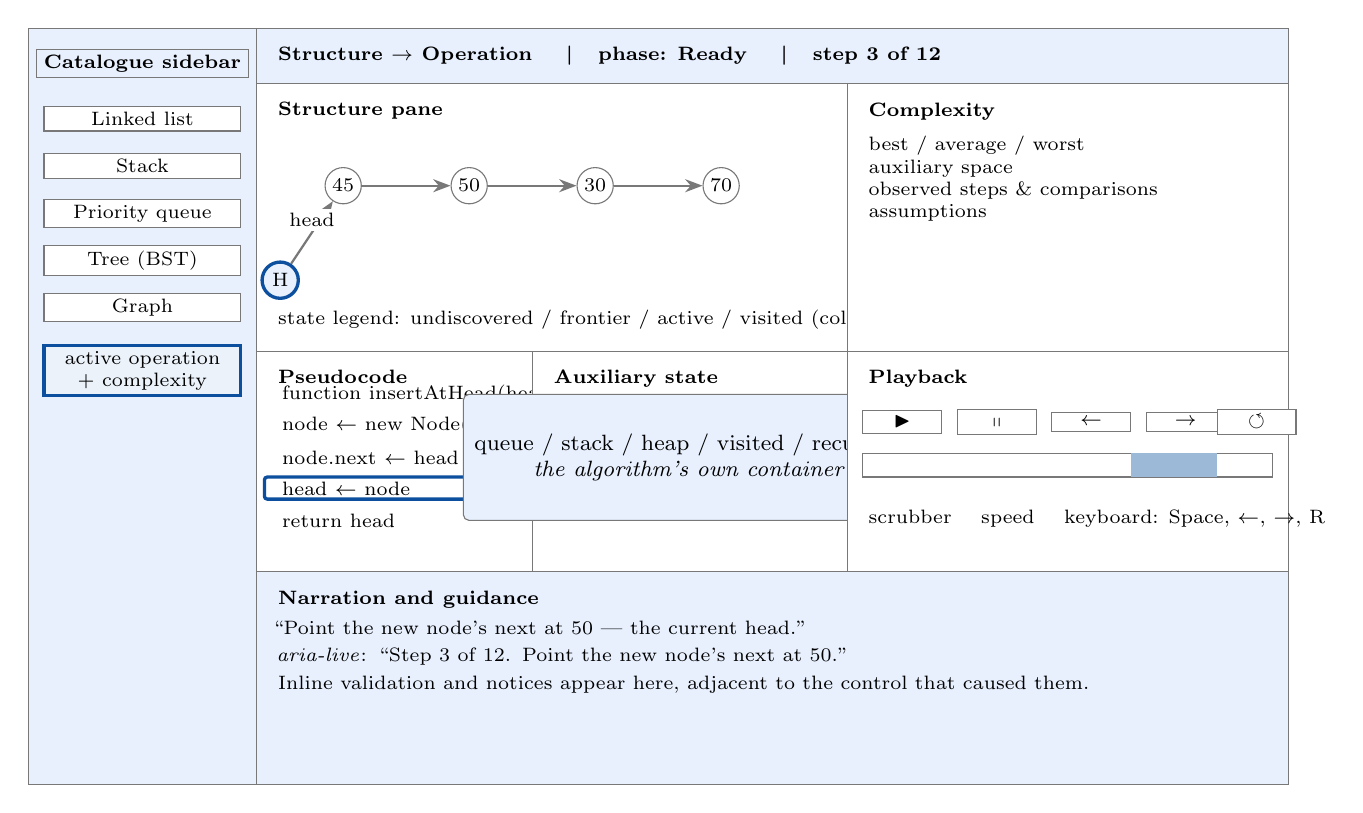
\begin{tikzpicture}[font=\scriptsize, x=1cm, y=1cm]
  % outer shell
  \draw[draw=rulec, fill=codec] (0,0) rectangle (16,9.6);
  % sidebar
  \draw[draw=rulec, fill=statec] (0,0) rectangle (2.9,9.6);
  \node[wfh, minimum width=2.7cm] at (1.45,9.15) {Catalogue sidebar};
  \node[wf, minimum width=2.5cm] at (1.45,8.45) {Linked list};
  \node[wf, minimum width=2.5cm] at (1.45,7.85) {Stack};
  \node[wf, minimum width=2.5cm] at (1.45,7.25) {Priority queue};
  \node[wf, minimum width=2.5cm] at (1.45,6.65) {Tree (BST)};
  \node[wf, minimum width=2.5cm] at (1.45,6.05) {Graph};
  \node[wf, minimum width=2.5cm, fill=boxc, draw=primary, very thick] at (1.45,5.25)
    {active operation\\ + complexity};
  % header
  \draw[draw=rulec, fill=statec] (2.9,8.9) rectangle (16,9.6);
  \node[anchor=west] at (3.05,9.25) {\bfseries Structure $\to$ Operation \quad
    \textbar\quad phase: Ready \quad \textbar\quad step 3 of 12};
  % structure pane
  \draw[wf] (2.9,5.5) rectangle (10.4,8.9);
  \node[anchor=north west] at (3.05,8.78) {\bfseries Structure pane};
  \node[n] (a) at (4.0,7.6) {45};
  \node[n] (b) at (5.6,7.6) {50};
  \node[n] (c) at (7.2,7.6) {30};
  \node[n] (d) at (8.8,7.6) {70};
  \draw[e] (a) -- (b); \draw[e] (b) -- (c); \draw[e] (c) -- (d);
  \node[nactive] (h) at (3.2,6.4) {H};
  \draw[e] (h) -- node[lbl,above]{head} (a);
  \node[anchor=south west] at (3.05,5.65) {state legend: undiscovered / frontier / active /
    visited (colour $+$ label)};
  % pseudocode pane
  \draw[wf] (2.9,2.7) rectangle (6.4,5.5);
  \node[anchor=north west] at (3.05,5.38) {\bfseries Pseudocode};
  \foreach \y/\t in {4.95/{function insertAtHead(head, value):},
                     4.55/{  node $\leftarrow$ new Node(value)},
                     4.15/{  node.next $\leftarrow$ head},
                     3.75/{  head $\leftarrow$ node},
                     3.35/{  return head}} {
    \node[anchor=west] at (3.1,\y) {\t};
  }
  \draw[draw=primary, very thick, rounded corners=1pt] (3.0,3.62) rectangle (6.3,3.9);
  % aux pane
  \draw[wf] (6.4,2.7) rectangle (10.4,5.5);
  \node[anchor=north west] at (6.55,5.38) {\bfseries Auxiliary state};
  \node[auxbox, minimum width=3.6cm, minimum height=1.6cm] at (8.4,4.15)
    {queue / stack / heap / visited / recursion\\ \emph{the algorithm's own container}};
  % complexity column
  \draw[wf] (10.4,5.5) rectangle (16,8.9);
  \node[anchor=north west] at (10.55,8.78) {\bfseries Complexity};
  \node[anchor=north west, align=left] at (10.55,8.35)
    {best / average / worst\\ auxiliary space\\ observed steps \& comparisons\\ assumptions};
  % controls column
  \draw[wf] (10.4,2.7) rectangle (16,5.5);
  \node[anchor=north west] at (10.55,5.38) {\bfseries Playback};
  \node[wf, minimum width=1.0cm] at (11.1,4.6) {$\blacktriangleright$};
  \node[wf, minimum width=1.0cm] at (12.3,4.6) {$\shortparallel$};
  \node[wf, minimum width=1.0cm] at (13.5,4.6) {$\leftarrow$};
  \node[wf, minimum width=1.0cm] at (14.7,4.6) {$\rightarrow$};
  \node[wf, minimum width=1.0cm] at (15.6,4.6) {$\circlearrowleft$};
  \draw[draw=rulec, fill=white] (10.6,3.9) rectangle (15.8,4.2);
  \fill[primary!40] (14.0,3.9) rectangle (15.1,4.2);
  \node[anchor=north west, align=left] at (10.55,3.6) {scrubber \quad speed \quad
    keyboard: Space, $\leftarrow$, $\rightarrow$, R};
  % narration bar
  \draw[draw=rulec, fill=statec] (2.9,0) rectangle (16,2.7);
  \node[anchor=north west] at (3.05,2.58) {\bfseries Narration and guidance};
  \node[anchor=north west, align=left, text width=12.1cm] at (3.05,2.2)
    {``Point the new node's next at 50 --- the current head.''\\[2pt]
     \emph{aria-live}: ``Step 3 of 12. Point the new node's next at 50.''\\[2pt]
     Inline validation and notices appear here, adjacent to the control that caused them.};
  % vertical divider labels
  \node[anchor=west] at (11.6,6.6) {};
\end{tikzpicture}
\caption{Wireframe of the operation workspace (V2). The sidebar and the narration bar persist;
the three panes are always the structure, the pseudocode and the auxiliary state at the same
index; the complexity card and the controls sit beside them. This is a wireframe: it fixes
regions and information, not styling.}
\label{fig:workspace}
\end{figure}

\begin{figure}[htbp]
\centering
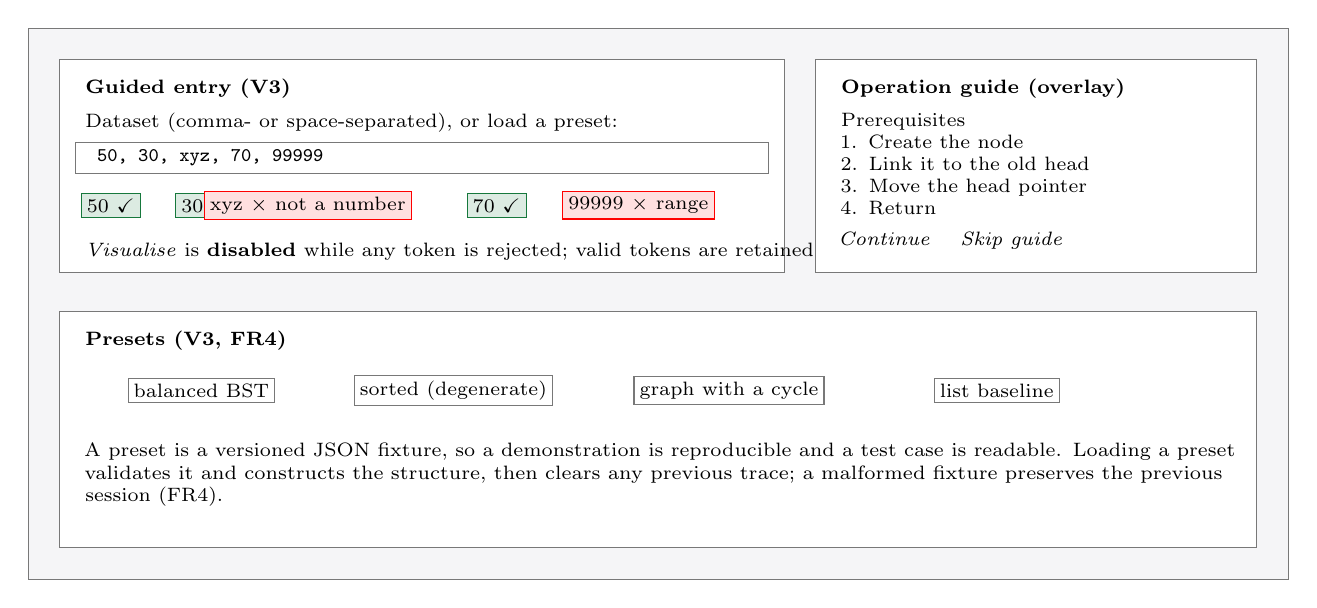
\begin{tikzpicture}[font=\scriptsize, x=1cm, y=1cm]
  \draw[draw=rulec, fill=codec] (0,0) rectangle (16,7.0);
  % entry card
  \draw[wf] (0.4,3.9) rectangle (9.6,6.6);
  \node[anchor=north west] at (0.6,6.48) {\bfseries Guided entry (V3)};
  \node[anchor=north west, align=left] at (0.6,6.05)
    {Dataset (comma- or space-separated), or load a preset:};
  \draw[draw=rulec, fill=white] (0.6,5.15) rectangle (9.4,5.55);
  \node[anchor=west] at (0.75,5.35) {\ct{50, 30, xyz, 70, 99999}};
  % token chips
  \node[wf, fill=okc!15, draw=okc]  at (1.05,4.75) {50 \checkmark};
  \node[wf, fill=okc!15, draw=okc]  at (2.25,4.75) {30 \checkmark};
  \node[wf, fill=red!12, draw=red]  at (3.55,4.75) {xyz $\times$ not a number};
  \node[wf, fill=okc!15, draw=okc]  at (5.95,4.75) {70 \checkmark};
  \node[wf, fill=red!12, draw=red]  at (7.75,4.75) {99999 $\times$ range};
  \node[anchor=north west, align=left] at (0.6,4.4)
    {\emph{Visualise} is \textbf{disabled} while any token is rejected; valid tokens are
     retained, so correcting the two bad ones is enough.};
  % guide overlay
  \draw[wf] (10.0,3.9) rectangle (15.6,6.6);
  \node[anchor=north west] at (10.2,6.48) {\bfseries Operation guide (overlay)};
  \node[anchor=north west, align=left, text width=5.1cm] at (10.2,6.05)
    {Prerequisites\\ 1. Create the node\\ 2. Link it to the old head\\ 3. Move the head
     pointer\\ 4. Return\\[3pt] \emph{Continue} \quad \emph{Skip guide}};
  % preset row
  \draw[wf] (0.4,0.4) rectangle (15.6,3.4);
  \node[anchor=north west] at (0.6,3.28) {\bfseries Presets (V3, FR4)};
  \node[wf] at (2.2,2.4) {balanced BST};
  \node[wf] at (5.4,2.4) {sorted (degenerate)};
  \node[wf] at (8.9,2.4) {graph with a cycle};
  \node[wf] at (12.3,2.4) {list baseline};
  \node[anchor=north west, align=left, text width=14.6cm] at (0.6,1.85)
    {A preset is a versioned JSON fixture, so a demonstration is reproducible and a test case
     is readable. Loading a preset validates it and constructs the structure, then clears any
     previous trace; a malformed fixture preserves the previous session (FR4).};
\end{tikzpicture}
\caption{Wireframe of the guided entry and presets (V3). Validation feedback is per token and
adjacent to the input; the operation guide is an overlay so the workspace is never lost.}
\label{fig:entry}
\end{figure}

\begin{figure}[htbp]
\centering
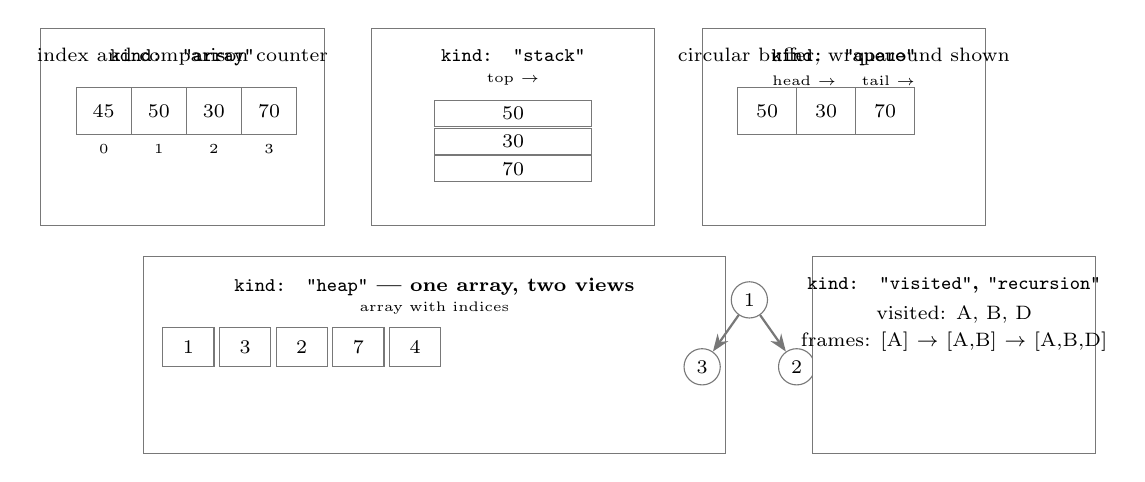
\begin{tikzpicture}[font=\scriptsize, x=1cm, y=1cm]
  % array
  \node[wf, minimum width=3.6cm, minimum height=2.5cm] (arr) at (2.2,4.4) {};
  \node[anchor=north] at (2.2,5.5) {\bfseries \ct{kind: "array"}};
  \foreach \x/\v in {0/45, 1/50, 2/30, 3/70} {
    \draw[draw=rulec, fill=white] (0.85+\x*0.7,4.3) rectangle (1.55+\x*0.7,4.9);
    \node at (1.2+\x*0.7,4.6) {\v};
    \node[font=\tiny] at (1.2+\x*0.7,4.12) {\x};
  }
  \node[anchor=south] at (2.2,5.05) {index and comparison counter};
  % stack
  \node[wf, minimum width=3.6cm, minimum height=2.5cm] (st) at (6.4,4.4) {};
  \node[anchor=north] at (6.4,5.5) {\bfseries \ct{kind: "stack"}};
  \foreach \y/\v in {3.7/70, 4.05/30, 4.4/50} {
    \draw[draw=rulec, fill=white] (5.4,\y) rectangle (7.4,\y+0.33);
    \node at (6.4,\y+0.165) {\v};
  }
  \node[anchor=south, font=\tiny] at (6.4,4.8) {top $\to$};
  % queue circular buffer
  \node[wf, minimum width=3.6cm, minimum height=2.5cm] (q) at (10.6,4.4) {};
  \node[anchor=north] at (10.6,5.5) {\bfseries \ct{kind: "queue"}};
  \foreach \x/\v in {0/50, 1/30, 2/70} {
    \draw[draw=rulec, fill=white] (9.25+\x*0.75,4.3) rectangle (10.0+\x*0.75,4.9);
    \node at (9.625+\x*0.75,4.6) {\v};
  }
  \node[anchor=south, font=\tiny] at (10.6,4.8) {head $\to$ \quad tail $\to$};
  \node[anchor=south] at (10.6,5.05) {circular buffer, wraparound shown};
  % heap
  \node[wf, minimum width=7.4cm, minimum height=2.5cm] (hp) at (5.4,1.5) {};
  \node[anchor=north] at (5.4,2.6) {\bfseries \ct{kind: "heap"} --- one array, two views};
  \foreach \x/\v in {0/1, 1/3, 2/2, 3/7, 4/4} {
    \draw[draw=rulec, fill=white] (1.95+\x*0.72,1.35) rectangle (2.6+\x*0.72,1.85);
    \node at (2.275+\x*0.72,1.6) {\v};
  }
  \node[n] (h0) at (9.4,2.2) {1};
  \node[n] (h1) at (8.8,1.35) {3};
  \node[n] (h2) at (10.0,1.35) {2};
  \draw[e] (h0) -- (h1); \draw[e] (h0) -- (h2);
  \node[anchor=south, font=\tiny] at (5.4,1.9) {array with indices};
  % visited / recursion
  \node[wf, minimum width=3.6cm, minimum height=2.5cm] (vis) at (12.0,1.5) {};
  \node[anchor=north] at (12.0,2.6) {\bfseries \ct{kind: "visited"}, \ct{"recursion"}};
  \node[anchor=north, align=center] at (12.0,2.25)
    {visited: A, B, D\\[2pt] frames: [A] $\to$ [A,B] $\to$ [A,B,D]};
\end{tikzpicture}
\caption{The auxiliary panel is one component per \ct{aux.kind} (FR10). The heap is shown
simultaneously as an array and as a complete binary tree, from one model, so the two views
cannot disagree; the queue shows its circular-buffer head and tail.}
\label{fig:aux}
\end{figure}

\subsection{Controls}

\A\ Table~\ref{tab:controls} is the control inventory. Every control maps to a requirement and
to a controller command; every keyboard binding maps to the same command as the
corresponding button.

{\footnotesize
\setlength{\tabcolsep}{4pt}
\begin{longtable}{@{}L{3.0cm}L{4.0cm}L{3.0cm}L{3.3cm}@{}}
\caption{Control inventory. ``Binding'' names the keyboard key where one exists; the keyboard
and the button invoke the same controller command.}\label{tab:controls}\\
\toprule
\textbf{Control} & \textbf{Action} & \textbf{Feedback} & \textbf{Binding / requirement} \\
\midrule
\endfirsthead
\toprule
\textbf{Control} & \textbf{Action} & \textbf{Feedback} & \textbf{Binding / requirement} \\
\midrule
\endhead
\bottomrule
\endlastfoot
Structure list & Select a structure; open its landing panel & Sidebar highlights the
selection; landing panel updates & Click; FR1 \\
Operation list & Select an operation; open V3 & Operation guide and complexity card load &
Click; FR2, FR3 \\
Preset selector & Load a curated dataset & Structure renders at step~0; preset name shown;
trace cleared & Click; FR4, FR13 \\
Values field & Type or paste values & Per-token chips with reasons; preview of accepted
dataset & Type; FR5, FR6 \\
Target field & Provide a search/delete key & Validated as a single value & Type; FR5 \\
\emph{Visualise} & Validate, build, execute, load & Disabled while input is invalid; success
loads step~0 & Click or Enter; FR7 \\
\emph{Play} / \emph{Pause} & Start / stop the single timer & Phase label; controls enable and
disable; step counter advances & Button or Space; FR11, NFR-U2 \\
\emph{Step back} / \emph{Step forward} & Move the index by $\pm 1$, clamped & Panes update;
narration and live region update; control disabled at the bound & Buttons or
$\leftarrow$ / $\rightarrow$; FR11 \\
\emph{Restart} & Index to $0$, phase to READY & Panes return to step~0; trace not recomputed &
Button or \ct{R}; FR13 \\
Speed & Change the step interval & The new rate applies from the next step & Selector;
FR11 \\
Scrubber & Seek to an arbitrary index & A frame is reconstructed from the nearest checkpoint &
Drag; FR11 \\
Panel collapse & Hide/show a pane & Layout remembers the preference (localStorage) &
Click; FR8--FR10 \\
\end{longtable}
}

\subsection{User workflow}

\R\ The workflow follows UC1 $\to$ UC2 and the five-stage pipeline of Assignment~2 \S5.3, and is
front-loaded so that the animation confirms an expectation rather than substituting for one.

\begin{enumerate}[leftmargin=1.6em,topsep=2pt,itemsep=1pt]
  \item \textbf{Orient and choose} (V1 $\to$ V3): the catalogue opens on a populated workspace
        (a default preset and trace), and selecting an operation opens its guide and complexity
        card before anything runs.
  \item \textbf{Supply data} (V3): keep a preset or type values and an optional target; every
        token is classified immediately and the preview shows exactly what will be used.
  \item \textbf{Visualise} (V3 $\to$ V2): the pipeline runs (parse $\to$ validate $\to$ build
        $\to$ execute $\to$ \ct{controller.load}); the workspace shows step~0 in READY.
  \item \textbf{Explore} (V2): play, pause, step, scrub and restart are all operations on one
        index, with narration, live region and the complexity card tracking each step.
  \item \textbf{Compare and recover} (V2/V3): change the preset or algorithm to compare runs,
        or correct rejected input and re-run --- an illegal operation is a disabled control with
        a reason, never a failure.
\end{enumerate}

\subsection{Feedback for successful operations}

\A\ Feedback is placed next to the thing it describes. \emph{Before execution} the complexity
card states the best/average/worst time and auxiliary space with assumptions in words, and the
guide has said what will happen. \emph{On each step} the narration bar gives one plain-English
sentence, the pseudocode highlights the executing line, the structure highlights the active
node and pointer, the auxiliary panel shows the algorithm's own container with the change since
the previous step emphasised, and the counter reads ``step $i$ of $n$''; the live region
announces the same text (NFR-U2, NFR-U3). \emph{On completion} the last step says what changed
and why it cost what it cost, the card shows observed against theoretical counts, and the final
structure is the confirmable result. Changing a preset or algorithm leaves both runs
inspectable, so a difference is a number and a picture rather than an assertion.

\subsection{Feedback for errors and invalid input}

\R\ ER1--ER13 define the behaviour; Table~\ref{tab:feedback} states where the user sees it. The
principle is that an error is a message about the algorithm, phrased in the user's domain ---
not a stack trace, and not a silent no-op.

\begin{table}[H]
\centering
\small
\setlength{\tabcolsep}{4pt}
\begin{tabular}{@{}L{2.4cm}L{4.0cm}L{3.4cm}L{3.5cm}@{}}
\toprule
\textbf{Situation} & \textbf{What the user sees} & \textbf{Placement} & \textbf{Recovery} \\
\midrule
Non-integer or out-of-range token (ER1, ER2) & The token is marked with its reason; valid
tokens are kept & Inline beside the field, per token & Edit the token; \emph{Visualise}
re-enables automatically \\
Empty or all-invalid dataset (ER3) & Empty-state hint with a valid example; \emph{Visualise}
disabled & Under the field & Provide values \\
Duplicate key (ER4) & The walk is shown; ``equal --- skipped'' notice & Notice region, next to
the workspace & Run continues; the user may remove the duplicate \\
Absent search/delete target (ER5) & The examined path stays highlighted; a ``not present''
banner & Notice region & Run completes; full cost is visible \\
Empty stack / queue (ER6) & Control disabled with a tooltip; keyboard command ignored with an
explicit message & On the control and in the notice region & No state change; run continues \\
Capacity exceeded (ER7) & Refusal names the capacity; capacity badge highlighted; auto-grow
note & On the structure and the notice region & Run continues with existing contents \\
Too many tokens (ER8) & Whole batch refused, with count and limit; nothing partial loaded &
Under the field & Split the input or use a preset \\
Malformed graph (ER9) & Per-line error list; previous graph untouched & Under the edge-list
field, per line & Fix the lines; load is atomic \\
Unreachable vertices (ER10) & ``$k$ of $n$ vertices reachable from \ct{A}''; component muted &
Notice region and structure pane & Restart from another source \\
Trace truncation (ER11) & Banner: trace truncated at the budget; reduce input & Above the
workspace & Reduce input \\
Rapid play/pause (ER12) & No visible error; commands coalesce & --- & Idempotent commands \\
Panel render failure (ER13) & The pane shows a fallback with \emph{Reset visualiser}; other
panes stay usable & In the failing pane & Reset the pane or the session \\
\bottomrule
\end{tabular}
\caption{Error feedback: what the user sees, where it appears, and how the session recovers.
This is the interface form of the ER table of Assignment~1 \S3.3.}
\label{tab:feedback}
\end{table}

\noindent\textbf{Principles.} \A\ (i)~Errors are never modal for invalid \emph{data}: the user
keeps editing. (ii)~A message names the offending value and the reason, never ``invalid
input''. (iii)~Disabled is preferred to failing: if a control cannot succeed, it is disabled
with a reason. (iv)~Errors do not destroy context: a malformed graph or preset leaves the
previous session intact. (v)~Errors are announced to assistive technology as well as drawn.

\subsection{Responsiveness and layout}

\R\ NFR-Po2 fixes the layout: the workspace collapses to a stacked layout below 1024~px, the
sidebar to icons below 768~px, and the design target is a classroom projector at
$1280\times720$. \A\ The layout is desktop-first for that target, with a graceful narrow mode:
the full three-pane workspace of Figure~\ref{fig:workspace} above 1280~px; the complexity card
and controls below the panes at 1024--1280~px with no horizontal scroll; a stacked workspace
with a pinned narration bar at 768--1024~px; an icon sidebar with tabbed panes below 768~px (a
courtesy mode, not the target); a pan-and-zoom viewport with an explicit cap note above the
caps (NFR-S1); and internally scrolling narration and pseudocode, with the executing line
auto-scrolled into view (FR9), while the structure pane pans and zooms without reflowing the
algorithm's state.

\subsection{Accessibility and usability}

\R\ The target is WCAG~2.1 AA (NFR-U2). \A\ \emph{Keyboard}: every control is reachable and
operable, focus order follows visual order, and the keyboard path invokes the same controller
commands as the buttons. \emph{Announcements}: step changes update an ARIA live region, and
validation rejects and error notices are announced; the counter has a text label.
\emph{Perceivable state}: contrast at least 4.5:1 and node state carried by colour \emph{and} a
label or shape. \emph{Motion}: \ct{prefers-reduced-motion} replaces interpolation with
instantaneous steps, affecting only the view. \emph{Structure}: semantic landmarks and headings,
a focus-trapping guide overlay, and a focusable error-boundary fallback. \emph{Usability}:
NFR-U1 targets the UC1 $\to$ UC2 flow in under three minutes at 80\% success across five users;
a populated first paint, an in-context guide, presets and per-step narration support it, and
the five-user check runs in Phase~5.

%=======================================================================
\section{Risks, Assumptions, and Limitations}

The brief asks for at least three technical risks with a mitigation each, at least three
assumptions, and at least three anticipated limitations. We give eight, seven and eight
respectively, because the honest risks of this project are not all technical and not all
alike.

\subsection{Technical risks and mitigations}

{\footnotesize
\setlength{\tabcolsep}{4pt}
\begin{longtable}{@{}L{0.8cm}L{3.5cm}L{1.3cm}L{1.3cm}L{6.6cm}@{}}
\caption{Technical and delivery risks, with impact, likelihood and the mechanism that enforces
each mitigation.}\label{tab:risks}\\
\toprule
\textbf{ID} & \textbf{Risk} & \textbf{Impact} & \textbf{Likelihood} & \textbf{Mitigation and enforcement} \\
\midrule
\endfirsthead
\toprule
\textbf{ID} & \textbf{Risk} & \textbf{Impact} & \textbf{Likelihood} & \textbf{Mitigation and enforcement} \\
\midrule
\endhead
\bottomrule
\endlastfoot
R1 & \textbf{Scope:} five structures and their operations are a large surface for two people,
so the graded set is not finished by the deadline & High & Medium & Build one vertical slice
first (done), freeze the \ct{Step} contract (ADR-8), then add operations additively; each
operation is one generator \(+\)
one listing \(+\)
one catalogue record (NFR-S2). Phase gates in Section~7 make the remaining surface visible
weekly, and the contract freeze means a slip delays a feature, not the architecture \\
R2 & \textbf{Two rendering paradigms:} mixing D3's DOM mutation with React's rendering
produces stale elements or flicker, especially on step-back & High & Medium & ADR-2 is
absolute for the main visualisation: D3 computes geometry, React owns the SVG; \ct{d3-selection}
is not used for the main view; the step-back DOM-equality test of T12 fails if a stale element
survives \\
R3 & \textbf{Non-determinism:} an unseeded random layout or neighbour order makes traces
irreproducible, breaking golden tests and exact replay & High & Medium & No wall-clock and no
randomness in the core (ADR-8 D7); the neighbour order is fixed to adjacency insertion order
and displayed; \ct{d3-force} is relaxed once with a fixed seed and frozen; an ESLint rule bans
\ct{Math.random} in \ct{core/}; golden traces catch any drift (NFR-C2) \\
R4 & \textbf{Performance at the cap:} aggregate generation or SVG reconciliation exceeds the
frame or latency budget at $n = 200$ & Medium & Medium & Precompute the trace and replay it;
run large generation in a Web Worker; keep per-frame state $O(n)$ with stable keys and
memoised panes; freeze the force layout; measure the budgets in CI (\S3.9) and degrade to
pan-and-zoom or truncate with disclosure (ER11) \\
R5 & \textbf{Content drift:} the pseudocode listing, the \ct{codeLine} map and the complexity
card disagree with the generator after a change & Medium & Medium & One \ct{OperationMeta}
record is the single source for the label, the listing id and the bounds; a completeness test
asserts every operation has a listing and a full line map; the golden trace changes in the same
pull request (FR3, FR9) \\
R6 & \textbf{Per-structure bugs in the model:} an invariant (heap property, BST ordering,
acyclicity) silently breaks and the animation teaches something wrong & High & Medium &
Invariants are asserted at every step of every trace, not only at the end (NFR-C4); every
operation is checked against an independent reference and the C textbook functions (NFR-C1);
property tests cover randomised inputs \\
R7 & \textbf{Test rot in the UI:} interaction tests written against the visual design break on
every restyle, so the team starts skipping them & Medium & Medium & Locate by role, accessible
name and text, never by class or pixel; golden \emph{traces} are the stable regression
artefact; screenshot tests are deliberately not used; one E2E walkthrough, not many \\
R8 & \textbf{Browser/worker compatibility:} \ct{structuredClone}, Web Worker or modern
ES features are unavailable in an older browser used by a grader & Low & Low & Target the last
two versions of the major browsers (NFR-Po1); feature-detect the worker and fall back to
main-thread generation; the app remains a static bundle with no server dependency \\
\end{longtable}
}

\subsection{Assumptions}

\begin{itemize}[leftmargin=1.4em,topsep=2pt,itemsep=1pt]
  \item \textbf{A1. Graded scope.} \A\ Linked list, stack, priority queue, tree (BST) and graph
        are graded; the FIFO queue is supporting and the traversals plus BFS/DFS are the graded
        algorithms (Assignment~2 \S2.1, ADR-5). A promotion is additive.
  \item \textbf{A2. Small inputs by design.} \A\ Teaching-sized data ($\le 100$ linear,
        $\le 200$ tree/graph); large-scale streaming is out of scope (NFR-S1).
  \item \textbf{A3. A modern evergreen browser on a conventional machine.} \A\ A 2020-era
        laptop with 8~GB of RAM on the latest stable Chrome; the budgets of \S4 assume it.
  \item \textbf{A4. Standard, unweighted algorithms.} \A\ Unweighted BFS and DFS; weighted
        shortest paths, self-balancing trees and union--find are out of scope (Assignment~2
        \S3.8).
  \item \textbf{A5. Data, not code.} \A\ Input is values and an edge list, never executable
        content; no \ct{eval} and no server, so no injection or data-at-rest surface
        (NFR-Se1).
  \item \textbf{A6. Determinism is achievable and desirable.} \A\ A fixed neighbour order and a
        seeded or frozen layout make every trace byte-identical, which is what golden tests and
        exact replay require (NFR-C2).
  \item \textbf{A7. Two people work in parallel against one frozen interface.} \A\ The
        \ct{Step} contract (ADR-8) and the layer boundaries (NFR-M2) are the coordination
        mechanism; both members review before merge.
\end{itemize}

\subsection{Anticipated limitations}

\begin{itemize}[leftmargin=1.4em,topsep=2pt,itemsep=1pt]
  \item \textbf{L1. A teaching visualiser, not an algorithm library.} \A\ It visualises its own
        operations step by step; it does not accept arbitrary user code.
  \item \textbf{L2. No persistence, sharing or accounts.} \A\ Without a backend (NFR-Se1) a
        session is not saved or resumed; traces export only as a fixture file.
  \item \textbf{L3. Legibility and animation degrade above the caps.} \A\ Beyond the caps the
        SVG pan-and-zoom is a workaround; the interface states the cap rather than degrading
        silently (NFR-S1).
  \item \textbf{L4. ``Observed step count'' is a model charge.} \A\ It counts emitted events and
        comparisons, not CPU cycles, and the complexity card says so.
  \item \textbf{L5. Accessibility is self-audited to WCAG~2.1 AA, not certified.} \A\ A formal
        audit and an exhaustive screen-reader matrix are outside the assignment's scope.
  \item \textbf{L6. Mobile and touch are courtesy modes.} \A\ The target is a
        $1280 \times 720$ projector and a desktop pointer; narrow layouts stack but a
        first-class touch experience is not a goal.
  \item \textbf{L7. The C reference functions are reading aids and test oracles.} \A\ They are
        the textbook algorithms (Assignment~2 \S3), not the shipped implementation.
  \item \textbf{L8. The visualised algorithm set is fixed for this iteration.} \A\ Dijkstra,
        $A^{*}$, topological sort, SCC and self-balancing trees are excluded (Assignment~2
        \S3.8); some are additive later, none is promised now.
\end{itemize}

%=======================================================================
\section{Development Plan}

The brief lists six phases and asks for a short plan with responsibilities and expected
outcomes, and for a description of how Git/GitHub will be used for regular, meaningful
commits and collaborative development.

\subsection{Phases, responsibilities and outcomes}

\R\ Table~\ref{tab:phases} follows the brief's six phases and adds an exit criterion and a
status for each. \A\ Responsibility is split by layer, because that is where the frozen
interface already divides the work: one member owns the core domain (models, generators,
trace store, oracles), the other owns the application and presentation layers (validation
plumbing, controller, worker, renderers, panes, accessibility), and both own the contract and
integration. Splitting by layer rather than by structure is deliberate: it keeps one person's
edits from spanning the boundary that the other person is responsible for.

\begin{table}[H]
\centering
\small
\setlength{\tabcolsep}{4pt}
\begin{tabular}{@{}L{0.7cm}L{4.3cm}L{2.6cm}L{3.2cm}L{3.0cm}@{}}
\toprule
\textbf{\#} & \textbf{Work} & \textbf{Responsible} & \textbf{Expected outcome} &
\textbf{Exit criterion / status} \\
\midrule
1 & Review requirements and technical design; confirm scope and the frozen contract &
Both (joint) & Agreed scope, ADRs, and the trace contract at v1 &
\done\ ADR-8 accepted; A1/A2 frozen \\
2 & Core data structures and system layer: five models, trace store, validator, controller,
state machine, worker & P.\ Morindat (models, store); Y.\ Megenta (controller, state machine,
validator, worker) & Every structure and system component present and unit-tested, with the
list slice fully working &
Partial: list model, store, controller, state machine and validator done (25 core tests pass);
the other four models are typed stubs \\
3 & Algorithms and core functionality: list/stack/heap/BST operations, the four traversals,
BFS and DFS, with instrumentation and complexity metadata & P.\ Morindat (generators); Y.\
Megenta (catalogue content, pseudocode listings, line maps) & Every graded operation emits a
correct, deterministic \ct{Step[]} and has a golden trace &
Not started; the \ct{insertAtHead} generator is the template and the contract is frozen \\
4 & UI/UX integration: structure renderers and layout, the three panes, controls, guide,
validation feedback, accessibility & Y.\ Megenta (renderers, panes, controls, a11y); P.\
Morindat (layout geometry, worker client) & The workspace of Figure~\ref{fig:workspace}
driven entirely by \ct{(trace, index)} &
Partial: shell, panes and list renderer exist for the slice; the other renderers and the full
control set are scheduled \\
5 & Testing and debugging: property and differential tests, integration, UI tests, golden
traces, performance budgets & Both, cross-reviewing & The suite of Section~3 green in CI, with
coverage at or above 90\% on \ct{src/core/**} &
Not started beyond the slice's 25 tests \\
6 & Final refinement and documentation: accessibility pass, usability check, README and ADR
updates, the demo script and the recorded walkthrough & Both (joint) & A demonstrable,
documented submission & Not started \\
\bottomrule
\end{tabular}
\caption{The six-phase development plan. ``Partial'' means the vertical slice satisfies part of
the phase; the status column is deliberately falsifiable against the repository.}
\label{tab:phases}
\end{table}

\subsection{Schedule and sequencing}

\A\ The plan is risk-first: the contract and the hardest integration points are settled early,
and the content that scales with the structure count is added last, when the pattern is
proven. Figure~\ref{fig:timeline} shows the six phases over six working weeks, with the
hardening phases overlapping the feature phases on purpose so that tests are written with
each feature rather than after all of them.

\begin{figure}[htbp]
\centering
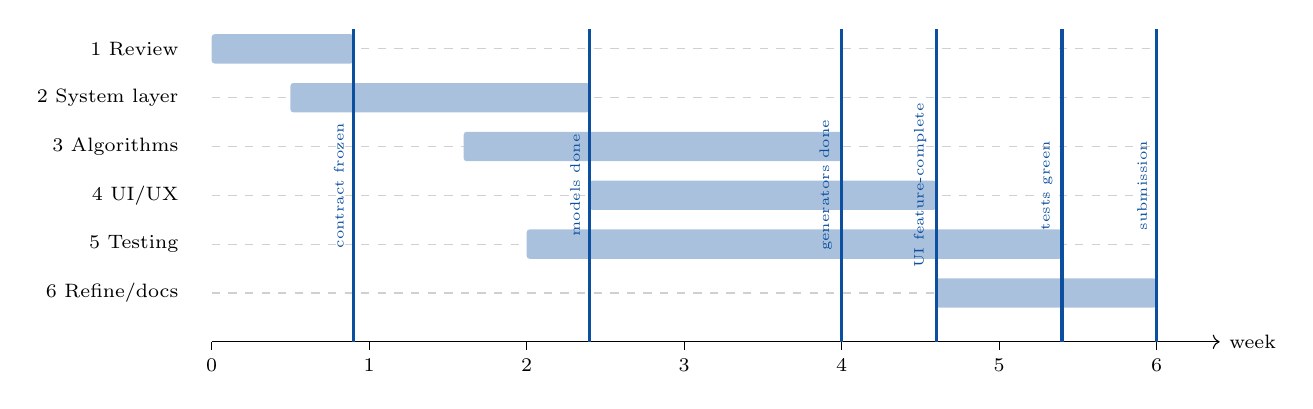
\begin{tikzpicture}[font=\scriptsize, x=2.0cm, y=0.62cm]
  % axes / weeks
  \draw[->] (0,0) -- (6.4,0) node[right]{week};
  \foreach \w in {0,1,2,3,4,5,6} {
    \draw (\w,0) -- (\w,-0.16);
    \node[below] at (\w,-0.16) {\w};
  }
  \foreach \y in {1,...,6} {
    \draw[rulec!35, dashed] (0,\y) -- (6,\y);
  }
  % labels
  \node[anchor=east] at (-0.15,6) {1 Review};
  \node[anchor=east] at (-0.15,5) {2 System layer};
  \node[anchor=east] at (-0.15,4) {3 Algorithms};
  \node[anchor=east] at (-0.15,3) {4 UI/UX};
  \node[anchor=east] at (-0.15,2) {5 Testing};
  \node[anchor=east] at (-0.15,1) {6 Refine/docs};
  % bars
  \fill[primary!35, rounded corners=1pt] (0.0,5.7) rectangle (0.9,6.3);
  \fill[primary!35, rounded corners=1pt] (0.5,4.7) rectangle (2.4,5.3);
  \fill[primary!35, rounded corners=1pt] (1.6,3.7) rectangle (4.0,4.3);
  \fill[primary!35, rounded corners=1pt] (2.4,2.7) rectangle (4.6,3.3);
  \fill[primary!35, rounded corners=1pt] (2.0,1.7) rectangle (5.4,2.3);
  \fill[primary!35, rounded corners=1pt] (4.6,0.7) rectangle (6.0,1.3);
  % milestones
  \foreach \x/\lab in {0.9/contract frozen, 2.4/models done, 4.0/generators done,
                       4.6/UI feature-complete, 5.4/tests green, 6.0/submission} {
    \draw[primary, very thick] (\x,0) -- (\x,6.4);
    \node[rotate=90, anchor=south, font=\tiny, text=primary] at (\x,3.2)
      {\lab};
  }
\end{tikzpicture}
\caption{Indicative schedule. Bars are the six phases; vertical lines are the gates that the
plan is actually managed against (the contract freeze is already met, so the plan starts
ahead on Phase~1).}
\label{fig:timeline}
\end{figure}

\subsection{Git and GitHub collaboration}

\R\ Instruction~5 makes the GitHub Classroom repository the submission channel; NFR-M1 and
NFR-M2 make quality enforcement part of the build. \A\ We use a trunk-based workflow with
short-lived branches and mandatory review, because it fits two people and keeps the frozen
contract under review.

\begin{itemize}[leftmargin=1.4em,topsep=2pt,itemsep=1pt,before=\raggedright]
  \item \textbf{\ct{main} is protected}: direct pushes are disabled, and a change lands only
        through a pull request with the other member's approval and all checks green.
  \item \textbf{Short-lived, single-purpose branches} (\ct{feat/bst-insert},
        \ct{test/heap-property}, \ct{docs/a3}, \ct{fix/checkpoint-replay}), merged or closed
        within a phase and deleted after merge.
  \item \textbf{Conventional, meaningful commits}, one logical change each, stating \emph{what}
        and \emph{why}: \ct{feat(bst): insert generator}, \ct{test(heap): heap invariant},
        \ct{docs(a3): testing plan}, \ct{refactor(trace): checkpoint search}.
  \item \textbf{A pull-request checklist}: does this change the \ct{Step} contract (if so, an
        ADR and regenerated golden traces)? does a new operation bring a generator, a listing
        and an \ct{OperationMeta}? are tests, coverage and docs green?
  \item \textbf{Contract changes are a deliberate, visible event} under the ADR-8 policy:
        additive changes bump the version note and regenerate the goldens; breaking changes
        update every producer and consumer and carry a migration note, in one commit;
        \ct{step.test.ts} locks the key set, so even an additive change needs approval. Golden
        traces are committed JSON and reviewed as diffs; \ct{--update} is never run blindly.
  \item \textbf{Issues, milestones and CI mirror the plan}: one issue per operation (acceptance
        criteria as in \S7.4), milestones are the six phases, labels distinguish
        \ct{area:core}, \ct{area:ui}, \ct{type:test}, \ct{type:docs} and \ct{risk}, and GitHub
        Actions runs \ct{typecheck}, \ct{lint}, \ct{test:core} and \ct{build} on every push
        (Phase~5 adds coverage, the payload budget and the E2E walkthrough).
  \item \textbf{Tagged checkpoints and docs with the code}: \ct{v0.1-slice},
        \ct{a3-submission} and phase tags make a demonstration reproducible; the README, the
        ADRs and the \LaTeX{} sources are version-controlled and updated in the same pull
        request as a behaviour change.
\end{itemize}

\subsection{Definition of done for an operation}

\A\ An operation is complete --- and therefore mergeable --- only when all of the following
hold. This is the same list as the PR checklist, in the form the team uses:

\begin{enumerate}[leftmargin=1.6em,topsep=2pt,itemsep=1pt]
  \item an instrumented generator in \ct{core/operations/} that emits a deterministic
        \ct{Step[]} and a \ct{GenerateSummary};
  \item an authored pseudocode listing and a total \ct{codeLine} map, plus its
        \ct{OperationMeta} record with best/average/worst/space and assumptions;
  \item unit tests for the step sequence, deltas and narration; an invariant assertion at
        every step; a reference/oracle test; and a golden-trace fixture;
  \item any new \ct{aux.kind} or renderer needed to display it;
  \item a documentation note if the complexity or the interface changed; and
  \item green CI on the pull request, with the other member's approval.
\end{enumerate}

%=======================================================================
\section{Expected Deliverables}

The brief asks what the final project will ultimately contain. Table~\ref{tab:deliverables}
lists the deliverables, the artefact a grader can inspect for each, and the phase that
produces it. The minimum list of the brief is covered, and four items are added that this
project specifically needs.

\begin{table}[H]
\centering
\small
\setlength{\tabcolsep}{4pt}
\begin{tabular}{@{}L{3.6cm}L{6.6cm}L{4.2cm}@{}}
\toprule
\textbf{Deliverable} & \textbf{What it is} & \textbf{Where / phase} \\
\midrule
Complete source code & Five structure models, the trace contract and store, the instrumented
generators for every graded operation, the traversals, BFS and DFS, the controller and
worker, the renderers and the UI, in the layered repository of Assignment~2 \S5.3 &
\ct{src/}; phases 2--4 \\
System and design documentation & The A1, A2 and A3 documents, the ADR set (including
ADR-8), and an up-to-date README with architecture and trace-contract sections &
\ct{ProjectResources/}, \ct{README.md}; all phases \\
Data representations & The \ct{Step}/\ct{StructureDelta}/\ct{AuxState} contract and the five
model representations, each with its invariants and its cost model & \ct{src/core/},
A2 \S4, A3 \S3--\S4 \\
Algorithm documentation & Per-operation pseudocode listings, the \ct{codeLine} maps, the C
reference functions, and the correctness intuitions of Assignment~2 \S3 &
\ct{src/data/catalogue.ts}, A2 \S3, A3 \S3.7 \\
Complexity analysis & The per-operation bound and auxiliary space, the trace-size and storage
bounds, and the observed-count comparison shown in the interface & A2 \S3--\S4, A3 \S4,
the complexity card \\
Demonstration of the major features & A live demonstration and a recorded walkthrough of the
UC1 $\to$ UC2 flow, a degenerate-versus-balanced BST comparison, a BFS/DFS comparison and a
heap build-versus-inserts comparison & Demo script and recording; phase 6 \\
Representative sample inputs & The versioned presets (balanced BST, sorted/degenerate BST,
graph with a cycle, list baseline) and the golden traces & \ct{src/data/presets/},
\ct{src/data/golden/}; phases 2--5 \\
Associated design assignments & This document and its two predecessors, compiled to PDF under
the required naming conventions & \ct{ProjectResources/}; continuous \\
\emph{Added:} test suite and quality evidence & The DOM-free core suite, property and oracle
tests, UI tests, one E2E walkthrough, golden traces, and the CI configuration that enforces
coverage and the import boundary & \ct{src/**/*.test.ts}, \ct{tests/}, \ct{.github/workflows/};
phases 4--5 \\
\emph{Added:} performance evidence & The budget harness results (generation latency, frame
time, payload, memory) against the \S4 targets & \ct{perf/} and CI; phase 5 \\
\emph{Added:} accessibility statement & A short statement of the WCAG~2.1 AA commitments, what
was tested, and the known limitations (L5) & \ct{README.md} and A3 \S5.8; phases 4--6 \\
\emph{Added:} a demo script & A reproducible path through the tool that exercises the graded
features in a fixed order, so a demonstration is not improvised & \ct{docs/demo.md}; phase 6 \\
\bottomrule
\end{tabular}
\caption{Expected final deliverables, the inspectable artefact, and the phase that produces
each.}
\label{tab:deliverables}
\end{table}

%=======================================================================
\section{Questions for Design Review}

\noindent The eight questions are answered concisely but technically.

\paragraph{1. What is the single most important algorithmic challenge in your project?}
\A\ Instrumenting the algorithms so the trace is \emph{complete and faithful} without changing
the cost model. For the graph searches this is sharpest: BFS and DFS are defined only up to the
order in which neighbours are expanded, so ``the correct trace'' does not exist until that order
is fixed, and a trace that omits the frontier at a dequeue hides exactly the state the learner
needs. We emit one step per meaningful event (dequeue/pop, examine-edge, discover, visit), carry
the algorithm's \emph{own} container in the step's \ct{aux} payload, and fix neighbours to
adjacency insertion order (Assignment~2 \S3.7). The challenge is then to show instrumentation adds
only $O(1)$ per step and that the instrumented result equals the textbook result --- which the C
reference oracle and the metamorphic tests of \S3.2 establish.

\paragraph{2. What is the most appropriate data structure for the central problem, and why?}
\A\ The central problem is not one of the five structures but making an execution addressable by
index, so the answer is the \textbf{immutable \ct{Step} plus a delta log with periodic
checkpoints}. \ct{Step} is snapshot-shaped for its readers, so the interface is a pure function
of \ct{(trace, index)}; the storage is a delta log, so memory is $O(s + (s/k)n)$ rather than
$O(ns)$ and display is independent of the index (ADR-1, ADR-3). The five models match their
textbook representations because that keeps the cost model honest, but the trace is what makes
the tool a visualiser rather than a library with a picture attached.

\paragraph{3. What is the most computationally expensive operation?}
\A\ Two, for different reasons. \emph{Trace generation for an aggregate session}: $n$ sorted BST
insertions produce $\Theta(n^2)$ steps on a degenerate tree ($\Theta(n\log n)$ balanced), each
also applied to the structure to keep generator and store in agreement. \emph{Per-frame rendering
at the cap}: at $n=200$ React reconciles $O(n)$ SVG elements which the browser lays out and
paints. Generation is offloaded to a Web Worker above the threshold, bounded by the step budget
and done once per run; rendering is bounded because no algorithm runs per frame, identifiers are
stable so React reuses DOM, and the force layout is relaxed once and frozen.

\paragraph{4. What happens when the user provides invalid input?}
\A\ Validation is total and precedes construction (ADR-7, FR6): every token is classified
independently and shown with a specific reason, valid tokens are retained, and \emph{Visualise}
is disabled while any token is invalid --- so no trace is generated and the engine is never
reached by raw text (asserted with a spy in \S3.6). Structure-specific rules apply on top:
duplicates are rejected on insert while the comparison walk is still shown (ER4); a graph load is
atomic and reports per-line errors (ER9); and a pop on an empty stack is a disabled control with
a reason, not an exception (ER6).

\paragraph{5. Which component is most likely to change during future development?}
\A\ The \emph{content and catalogue layer} --- pseudocode listings, \ct{codeLine} maps, guide
text and complexity records --- together with the set of \ct{aux} panel kinds and renderers. It
is the layer that grows with scope and the one a course would extend. The \ct{Step} contract was
frozen at v1 (ADR-8) precisely so that it is \emph{not} the churning component; it may grow
additively, but only as a deliberate, ADR-backed event.

\paragraph{6. How does your architecture isolate that component?}
\A\ Content is data, not code: one \ct{OperationMeta} and one pseudocode listing per operation,
read only through \ct{app/catalogue.ts}, so the UI holds no hard-coded bound or listing. Adding
an operation is exactly three edits --- one generator, one listing plus line map, one catalogue
record (Assignment~2 \S5.7, NFR-S2) --- and the controller, state machine and shell stay
untouched. The same isolation bounds \ct{aux} and renderer changes: the \ct{AuxKind} and
\ct{EdgeKind} unions are closed, one panel handles one kind, and a new structure needs one model
and one renderer. The import-boundary lint rule (NFR-M2) enforces the direction.

\paragraph{7. What is one design decision you considered but rejected? Why?}
\A\ \textbf{Recomputing the algorithm's state on demand instead of storing a trace.} It is
simpler to write, costs no storage and is correct for forward stepping, but every move ---
including step-back, which a learner relies on --- would cost $O(i)$, and state that depends on
the run so far (the exact BFS frontier, the recursion depth) could not be represented without
replaying that history. It makes the state \emph{recomputable} rather than \emph{addressable}, so
the UI could not scrub and a timing difference could change what the learner sees. A stored
deterministic trace costs one generation pass and $O(s)$ memory and makes step-back, scrub and
exact replay architectural (ADR-1). A second rejection, in one line: letting \ct{d3-selection}
own the main SVG is a known source of stale elements on step-back (ADR-2).

\paragraph{8. What additional feature could be implemented without redesigning the core
architecture?}
\A\ Several, which is the evidence that the design is extensible. \textbf{Topological sort,
cycle detection and SCC} reuse the DFS generator and add an edge-classification or post-order
rule (one generator, one listing). \textbf{Dijkstra} uses the already-graded priority queue as
its frontier and adds relaxation events. \textbf{Promoting the FIFO queue} to a catalogue entry
is one catalogue record, one generator set and one renderer, since its circular buffer and
\ct{aux.kind} already exist. \textbf{Expression-tree evaluation} is postorder plus an arithmetic
rule, and \textbf{exporting or deep-linking a trace} needs no engine change because the trace is
already serialisable. In every case the \ct{Step} contract, store, controller and shell are
unchanged.

%=======================================================================
\section{Submission Checklist}

Every item from the brief is listed with the section that satisfies it and the evidence a
grader should look for. Legend: \done\ satisfied in this document; \todo\ a team action
completed at submission time.

{\small
\setlength{\tabcolsep}{4pt}
\begin{longtable}{@{}C{0.7cm}L{6.4cm}L{2.3cm}L{5.6cm}@{}}
\toprule
& \textbf{Checklist item} & \textbf{Where satisfied} & \textbf{Evidence} \\
\midrule
\endfirsthead
\toprule
& \textbf{Checklist item} & \textbf{Where satisfied} & \textbf{Evidence} \\
\midrule
\endhead
\bottomrule
\endlastfoot

\done & Project title and team information are included. &
\S1, \S1.1 & The identification table with both members and roll numbers, the repository
link, and the project title, problem statement, motivation, users and goal. \\

\done & Testing strategy is documented. &
\S3.1--\S3.9 & Nine test levels with tools, scope and evidence; the strategy is stated as a
pyramid and each level is tied to a non-functional requirement. \\

\done & Representative test cases are included. &
\S3.10 & Thirteen cases (T1--T13) in the brief's Input / Expected output / Purpose form, with
T1 and T4 expanded in full; the set covers every category the brief names. \\

\done & Boundary and invalid-input cases are addressed. &
\S3.5, \S3.6 & A per-area boundary table and an ER1--ER13 invalid-input table, plus a
totality property test. \\

\done & Complexity and performance considerations are discussed. &
\S4 & Time and auxiliary space per operation, trace-size and storage bounds, the $O(n+k)$
display bound, expected input sizes, six named bottlenecks and their mitigations, and a
trade-off table. \\

\done & UI/UX design and user workflows are documented. &
\S5 & Six views, a control inventory, the seven-stage workflow, and four figures: workspace,
guided entry, auxiliary-panel variants and the workflow. \\

\done & Feedback and error-handling considerations are addressed. &
\S5.5--\S5.6 & Success feedback per phase of a run, and a table mapping ER1--ER13 to what the
user sees, where, and how the session recovers. \\

\done & Risks, assumptions, and limitations are identified. &
\S6 & Eight risks, seven assumptions and eight limitations --- above the brief's minimum of
three each. \\

\done & Risk mitigation strategies are provided. &
\S6.1 & Each risk has impact, likelihood and a mitigation with the mechanism that enforces
it (contract freeze, invariant tests, golden traces, Worker, CI budgets). \\

\done & Development plan and responsibilities are included. &
\S7.1--\S7.2 & The brief's six phases with responsible members, expected outcomes, exit
criteria and a current status, plus an indicative six-week schedule with gates. \\

\done & Git/GitHub collaboration practices are described. &
\S7.3--\S7.4 & Protected \ct{main}, short-lived branches, conventional commits, a PR
checklist, contract-change policy, issue/milestone mapping and a definition of done. \\

\done & Expected final project deliverables are identified. &
\S8 & Twelve deliverables (the brief's eight plus four), each with an inspectable artefact
and the phase that produces it. \\

\done & Design-review questions are answered. &
\S9 & All eight questions answered concisely and technically. \\

\done & The document is compiled successfully using \LaTeX. &
Build & This source, \ct{A3\_PY.tex}, compiles with \ct{tectonic -X compile A3\_PY.tex}. \\

\todo & The PDF follows the required naming convention. &
Title block & \textbf{Team action:} the compiled PDF is named \ct{A3\_PY.pdf}. \\

\done & All team members are listed. &
\S1 & Papaa Dennis Morindat (1020241748) and Yididiya Megenta (1020241852). \\

\end{longtable}
}

\paragraph{Additional self-checks before submitting.}
\begin{itemize}[leftmargin=1.6em,itemsep=2pt]
  \item Confirm that every \done\ in \S3.10 still matches the repository: a checkmark on a
        test that does not run is worse than no checkmark.
  \item Confirm that each test identifier quoted from Assignment~1 (FR, ER, NFR, UC) still
        refers to the same requirement, and that no \A{} has been promoted to an \R{}.
  \item Confirm that the status column of Table~\ref{tab:phases} and the ``current evidence''
        paragraph of \S3.11 agree with the state of \ct{main} on the day of submission.
  \item Re-run \ct{npm run check} on \ct{main} and record the result; the performance claims
        of \S4 are targets, and the document says so.
  \item Confirm that only Project~3 is discussed, as the brief requires.
\end{itemize}

%=======================================================================
\appendix
\section{Requirement-to-Test Traceability Matrix}

\A\ This appendix exists so that a grader can check coverage without reading the whole
document. Every requirement family of Assignment~1 appears with the tests, oracles and gates
that establish it.

\begin{table}[H]
\centering
\small
\setlength{\tabcolsep}{4pt}
\begin{tabular}{@{}L{2.5cm}L{6.0cm}L{4.0cm}L{3.0cm}@{}}
\toprule
\textbf{Requirement} & \textbf{Statement (abbreviated)} & \textbf{Tests / oracle} &
\textbf{Gate} \\
\midrule
FR6 & Validation is total; the engine never sees raw text & T3, \S3.6 totality property,
generator spy & L5, CI \\
FR7 & Trace generation is pure and deterministic & T1, T7, T9; golden traces; L3 oracles &
\ct{test:core}, golden diff \\
FR8--FR10 & Structure, pseudocode and auxiliary panes are functions of the step & T12; L7 UI
tests & CI (Phase~4) \\
FR11 & One controller, one timer, clamped and idempotent commands & T10; state-machine table &
\ct{test:core} \\
FR12 & BFS/DFS with a fixed, reproducible neighbour order & T7, T8; C oracle; reference BFS &
\ct{test:core}, golden \\
ER1--ER3 & Malformed, out-of-range and empty datasets & T3; \S3.6 table & L5 \\
ER4--ER5 & Duplicate insert; absent search/delete target & T4; algorithm tests & L2, L3 \\
ER6--ER7 & Underflow and overflow are outcomes, not exceptions & \S3.5; L1/L2 tests & CI \\
ER8--ER9 & Token cap; malformed graph load is atomic & T3, \S3.6 & L5 \\
ER10--ER11 & Reachability reported; pathological trace truncated & T7; step-budget test & L9 \\
ER12--ER13 & One timer under rapid input; panel failure contained & T10, T12 & L7 \\
NFR-C1 & Result equals an independent reference & L3; reference implementations; C oracle &
\ct{test:core} \\
NFR-C2 & Byte-identical trace for the same input & T1, T7, T9; golden traces & golden diff \\
NFR-C3 & Every malformed token rejected with a reason & T3, \S3.6 & L5 \\
NFR-C4 & Invariants hold at every step & T4, T6; invariant oracle & \ct{test:core} \\
NFR-P1--P5 & Payload, feedback, frame time, generation latency, memory & T13; budget harness;
Lighthouse & Phase~5 \\
NFR-U1 & First-time user completes UC1 $\to$ UC2 in three minutes & Five-user check; E2E
walkthrough & Phase~5 \\
NFR-U2--U3 & WCAG~2.1 AA, keyboard, live region, narration & T12; accessibility checklist of
\S5.8 & Phase~5 \\
NFR-S1 & Documented caps and disclosed degradation & \S4.3; cap and cap$+1$ boundary tests &
L9 \\
NFR-S2 & A new operation is one generator, one listing, one catalogue record & \S9.6,
\S9.8; catalogue completeness test & CI (Phase~3) \\
NFR-M1--M3 & Coverage, strict types, import boundary, one contract module & \S3.11 gates;
\ct{test:core} in Node; ESLint boundary & CI \\
NFR-Se2 & Resource safety: capped input, terminated worker & T11, T13; ER11 & CI (Phase~5) \\
UC1--UC7 & The seven use cases & T1--T13 collectively; the E2E walkthrough covers UC1, UC2 and
UC4 & Phase~5 \\
\bottomrule
\end{tabular}
\caption{Requirement-to-test traceability. ``Gate'' names the mechanism that makes the claim
continuously true rather than true once.}
\label{tab:trace}
\end{table}

\end{document}
